% template by Natalia Chernov for the University of Oldenburg

\documentclass[xcolor=table,9pt,aspectratio=169]{beamer}

\usepackage[utf8]{inputenc}

\usepackage{amsmath}
\usepackage{anyfontsize}
\usepackage[english]{babel}
\usepackage[autostyle]{csquotes}
\usepackage{datetime}
\usepackage{enumitem}
   \def\labelitemi{--}
   \def\labelitemii{--}
   \def\labelitemiii{--}
\usepackage{helvet}
   \renewcommand{\familydefault}{\sfdefault}
\usepackage{lipsum}
\usepackage{lmodern}
\usepackage{multicol}
\usepackage{smartdiagram}
\usepackage{tikz}

\definecolor{uolblue}{RGB}{0,62,107}

\definecolor{blue1}{RGB}{0,78,159}
\definecolor{blue2}{RGB}{0,171,217}
\definecolor{blue3}{RGB}{91,197,242}
\definecolor{blue4}{RGB}{161,217,248}

\definecolor{green1}{RGB}{0,120,120}
\definecolor{green2}{RGB}{0,168,121}
\definecolor{green3}{RGB}{148,193,28}
\definecolor{green4}{RGB}{199,211,0}

\definecolor{orange1}{RGB}{213,59,10}
\definecolor{orange2}{RGB}{238,113,0}
\definecolor{orange3}{RGB}{243,145,0}
\definecolor{orange4}{RGB}{253,195,0}

\definecolor{gr}{RGB}{191,191,191}

\setbeameroption{hide notes}
% \setbeameroption{show only notes}
% \setbeameroption{show notes on second screen=right}

\setbeamertemplate{frametitle}{\color{uolblue}\fontsize{12}{20}\selectfont{\insertframetitle}}

\pgfdeclareimage[width=0.145\paperwidth]{logo}{figures/slides_logo_uol_negative}
\pgfdeclareimage[width=0.072\paperwidth]{logo_small}{figures/slides_logo_uol_negative}

\defbeamertemplate*{background canvas}{default_page}
{%
\begin{tikzpicture}
   \useasboundingbox (0,0) rectangle (\the\paperwidth,\the\paperheight);
   \filldraw[fill=uolblue,fill opacity=1,draw=none] (0,0) rectangle (0.119\paperwidth,\the\paperheight);
   \filldraw[fill=blue2,fill opacity=1,draw=none] (0.119\paperwidth,0) -- (0.119\paperwidth,0.565\paperheight) arc (117.2:180:0.6\paperwidth) -- cycle;
   \pgftext[at=\pgfpoint{10}{\the\paperheight-11.5},left,top]{\pgfsetfillopacity{1}\pgfuseimage{logo_small}};
\end{tikzpicture}
}
\defbeamertemplate*{background canvas}{titlepage_image}
{
\begin{tikzpicture}
   \useasboundingbox (0,0) rectangle (\the\paperwidth,\the\paperheight);
   \filldraw[fill=uolblue,fill opacity=1,draw=none] (0,0) rectangle (\the\paperwidth,\the\paperheight);
   \filldraw[fill=blue2,fill opacity=1,draw=none] (\the\paperwidth,0) -- (\the\paperwidth,0.66\paperheight) arc (90:180:0.6\paperwidth) -- cycle;
   \pgftext[at=\pgfpoint{14}{\the\paperheight-17.5},left,top]{\pgfsetfillopacity{1}\pgfuseimage{logo}};
\end{tikzpicture}
}
\BeforeBeginEnvironment{frame}{%
   \setbeamertemplate{background canvas}[default_page]%
}
\makeatletter
\define@key{beamerframe}{titlepage_image}[true]{%
   \setbeamercovered{invisible}%
   \setbeamertemplate{background canvas}[titlepage_image]%
}
\makeatother%

\setbeamertemplate{footline}
{
   \leavevmode
   \hbox{
   \hspace*{.025\paperwidth}\begin{beamercolorbox}[wd=.094\paperwidth,ht=2.25ex,dp=1ex,left]{}
   ~

   \vspace*{.042\paperheight}
      \fontsize{4.4}{5.9}\selectfont\color{white}\textbf{Slide \insertframenumber}\newline\insertdate
   \vspace*{.026\paperheight}
   \end{beamercolorbox}
   \hspace*{.05\paperwidth}\begin{beamercolorbox}
   [wd=.79\paperwidth,ht=2.25ex,dp=1ex,left]{}
   ~

   \vspace*{.042\paperheight}
      \fontsize{4.4}{5.9}\selectfont\color{black}\textbf{Empirical Studies on Questions of Need-Based Distributive Justice}\newline\color{gray}\insertauthor~--~School of Humanities and Social Sciences, Department of Philosophy
   \vspace*{.026\paperheight}
   \end{beamercolorbox}
   }
   \vskip0pt
}

\setbeamerfont{title}{size={\fontsize{22}{25}}}
\setbeamerfont{subtitle}{size={\fontsize{12}{14}}}
\setbeamerfont{author}{size={\fontsize{9}{11}}}
\setbeamerfont{date}{size={\fontsize{9}{11}}}
\setbeamercolor{title}{fg=white}
\setbeamercolor{subtitle}{fg=white}
\setbeamercolor{author}{fg=white}
\setbeamercolor{date}{fg=white}
\setbeamercolor{color_Logo-Platzhalter}{fg=white,bg=gray!40}

\defbeamertemplate*{title page}{customized}[1][]
{  \vspace*{20mm}
   \hspace*{-22.5mm}
   \begin{minipage}{\textwidth}
   \usebeamerfont{title}\usebeamercolor[fg]{title}\inserttitle\par
   \bigskip
   \usebeamerfont{subtitle}\usebeamercolor[fg]{subtitle}\insertsubtitle\par
   \bigskip
   \usebeamerfont{author}\usebeamercolor[fg]{author}\insertauthor\par
   \bigskip
   \usebeamerfont{date}\usebeamercolor[fg]{date}\insertdate\par
   \end{minipage}
}
\setbeamertemplate{navigation symbols}{}
\setbeamersize{text margin left=0.17\paperwidth,text margin right=0.04\paperwidth}

\title{Empirical Studies on Questions of\\ Need-Based Distributive Justice}
\subtitle{}
\author{Alexander Max Bauer}
\date{July 12, 2025}
% \date{\renewcommand{\dateseparator}{.}\ddmmyyyydate\today}

\begin{document}
{
\setbeamertemplate{footline}{}
\begin{frame}[titlepage_image]
   \maketitle
\end{frame}
}


%%%%%%%%%%%%%%%%%%%%%%
% SLIDE 2 – FOR 2104 %
%%%%%%%%%%%%%%%%%%%%%%
\begin{frame}{\vspace*{10mm}}
\frame{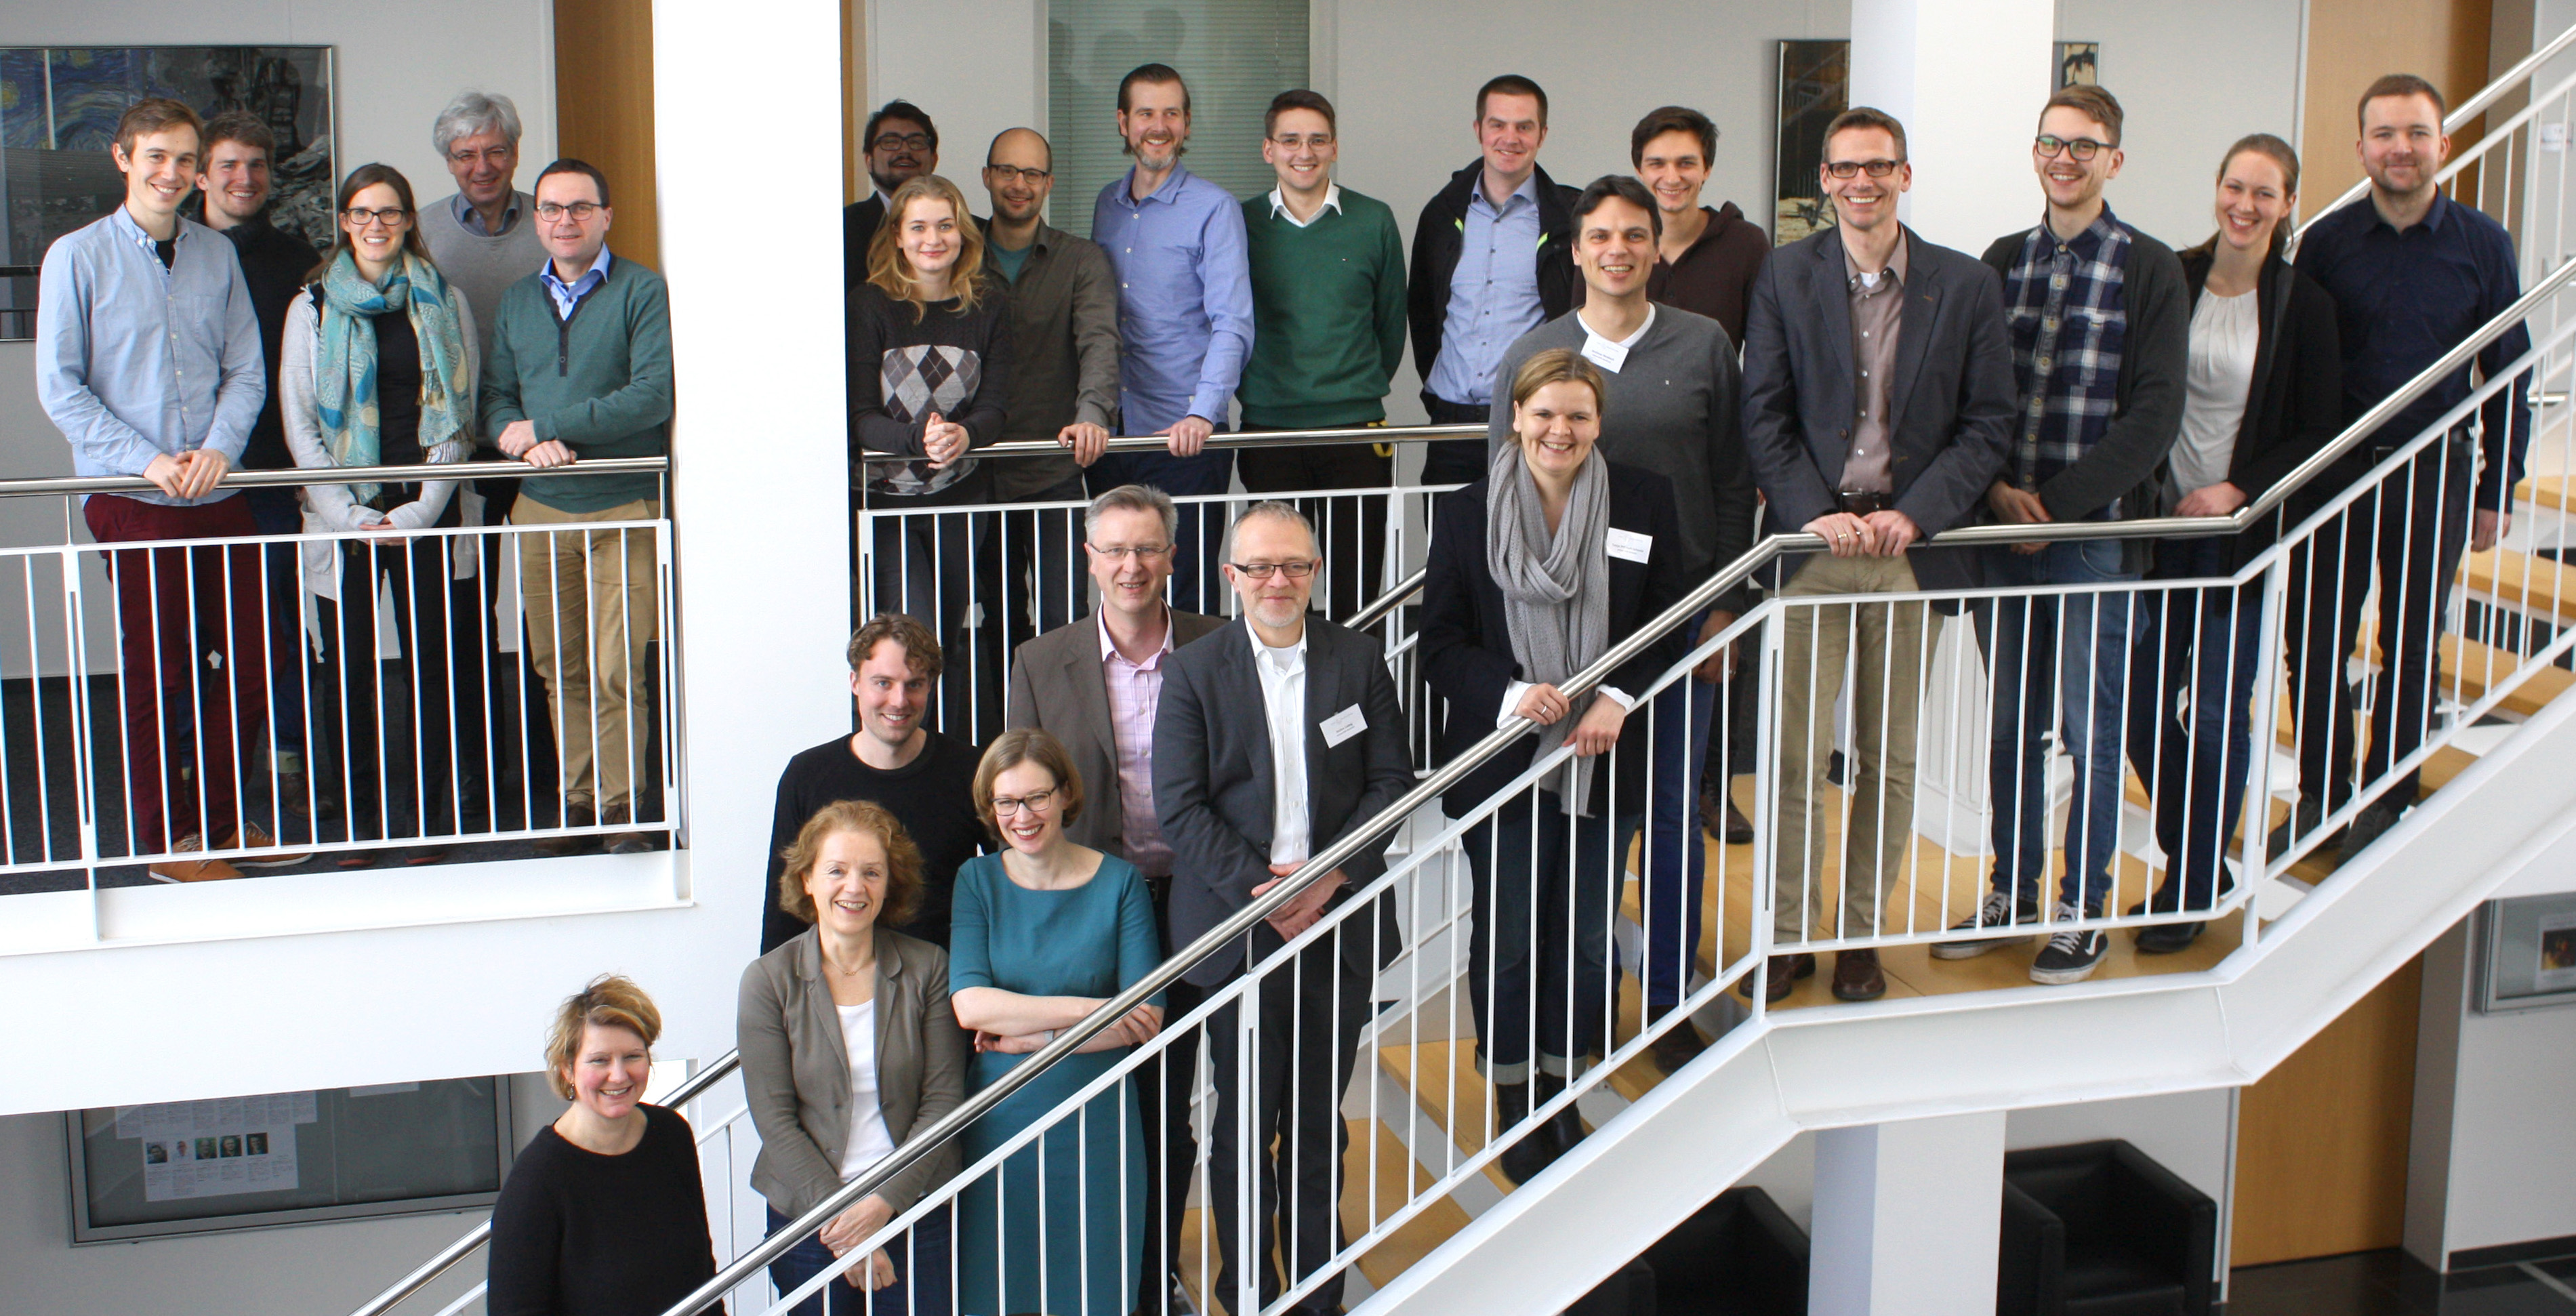
\includegraphics[width=1\linewidth]{figures/slides_for.jpg}}
\note{
   \begin{itemize}
      \item FOR 2104 \enquote{Need-Based Justice and Distribution Procedures}
      \item A2 \enquote{Measures of Need-Based Distributive Justice, Expertise, and Coherence}
      \item Hanse-Wissenschaftskolleg Delmenhorst 2017
   \end{itemize}
}
\end{frame}


%%%%%%%%%%%%%%%%%%
% SLIDE 3 – TEAM %
%%%%%%%%%%%%%%%%%%
\begin{frame}{}

\includegraphics[width=1\linewidth]{figures/slides_team.pdf}
\end{frame}


%%%%%%%%%%%%%%%%%%%%%
% SLIDE 4 – ROADMAP %
%%%%%%%%%%%%%%%%%%%%%
\begin{frame}{\vspace*{10mm}Roadmap}
\begin{itemize}
   \item[1] \hspace*{1em}Need as Reference Point \textcolor{gray}{(Bauer et al. forthcoming)}
   \item[2] \hspace*{1em}Need and Accountability \textcolor{gray}{(Bauer et al. 2022, Bauer and Romann 2024)}
   \item[3] \hspace*{1em}Kinds of Needs \textcolor{gray}{(Bauer et al. 2023)}
   \begin{itemize}
      \item[3.1] \hspace*{1em}Study 1
      \item[3.2] \hspace*{1em}Study 2
   \end{itemize}
   \item[4] \hspace*{1em}Summary of Key Results
\end{itemize}
\end{frame}


%%%%%%%%%%%%%%%%%%%%%%%%%%%%%%%%%%%%%
% SLIDE 5 – NEED AS REFERENCE POINT %
%%%%%%%%%%%%%%%%%%%%%%%%%%%%%%%%%%%%%
\begin{frame}
\begin{overlayarea}{\textwidth}{0.81\paperheight}{
   \vspace*{11mm}
   \usebeamerfont{title}\textcolor{uolblue}
   {1\hspace*{1em}Need as Reference Point}
}
\end{overlayarea}
\end{frame}


%%%%%%%%%%%
% SLIDE 6 %
%%%%%%%%%%%
\begin{frame}{\vspace*{10mm}1\hspace*{1em}Need as Reference Point}
\begin{multicols}{2}
   \textbf{Background}\\
   \medskip
   \begin{itemize}
      \item People make gradual evaluations of the justice of distribution scenarios
      \item Is there a connection between the evaluation of justice and meeting needs? What role does a needs threshold play in this?
   \end{itemize}
   \vfill
   \begin{center}
      \frame{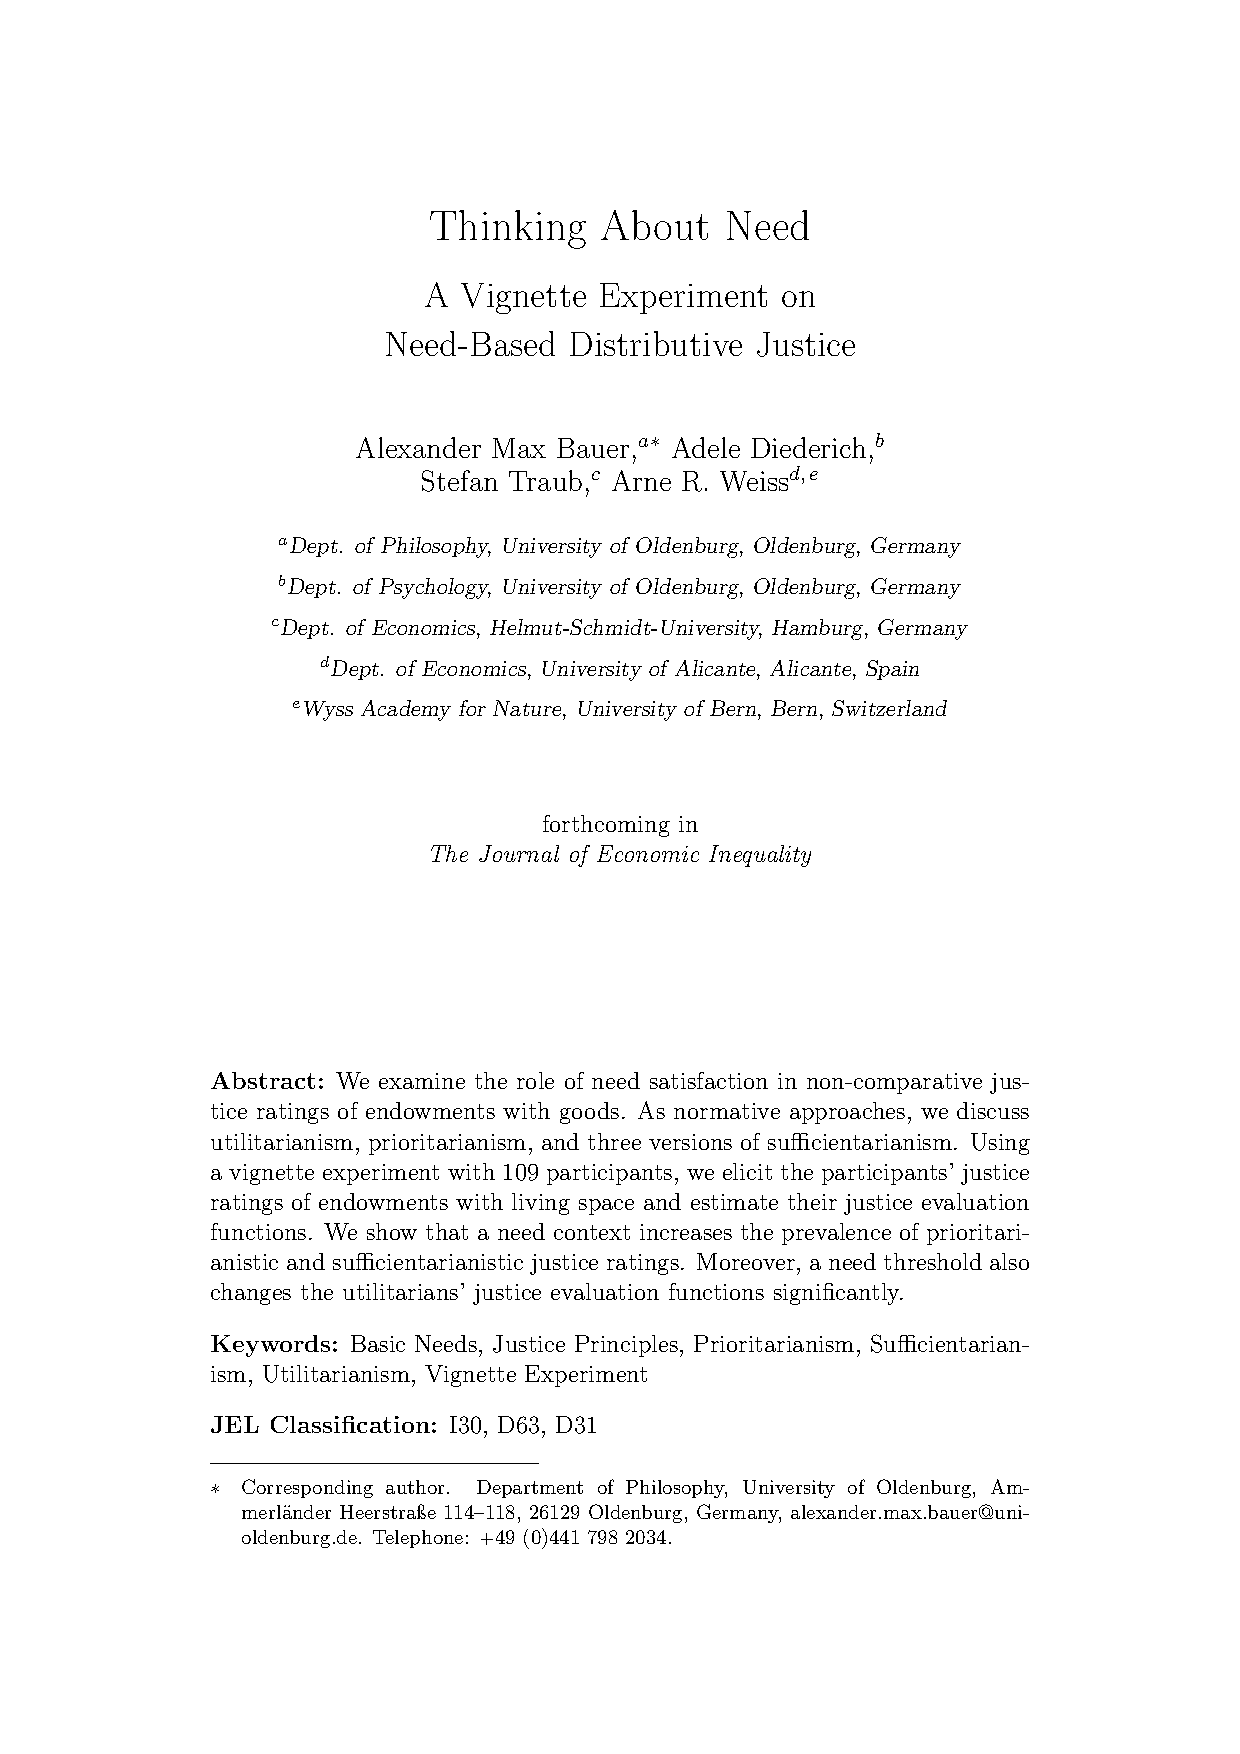
\includegraphics[width=0.6\linewidth]{figures/slides_bauer_et_al_forthcoming.pdf}}\\
      \textcolor{gray}{Bauer et al. forthcoming}
   \end{center}
\end{multicols}
\end{frame}


%%%%%%%%%%%
% SLIDE 7 %
%%%%%%%%%%%
\begin{frame}{\vspace*{10mm}1\hspace*{1em}Need as Reference Point}
\textbf{Design and Implementation}\\
\medskip
\begin{itemize}
   \item WiSo Lab, University of Hamburg, September 2016
   \item $n=116$
   \item Impartial observers
   \item Need and Control Group (\textit{between subjects})
   \item Global and Relative Evaluation Task (\textit{within subjects})
   \item $11$ cases
\end{itemize}
\end{frame}


%%%%%%%%%%%
% SLIDE 8 %
%%%%%%%%%%%
\begin{frame}{\vspace*{10mm}1\hspace*{1em}Need as Reference Point}
\textbf{Vignette (1/2)}\\
\medskip
\enquote{Please imagine the following:\\
\medskip
In the region of Bergtal, a new village is going to be established.
It is the task of the Public Housing Association of Bergtal to build housing.\\
\medskip
All households in this region want to live in the largest living space possible.
\textcolor{blue1}{The residents of the region have collectively decided on a minimum amount of living space, under which living a decent life in this community is not possible.}
Between the households in the region, there are no noteworthy differences \textcolor{blue1}{and the minimum amounts are the same for each household:
Each household should have 1000 regional---i.\,e., common to the region---area units of living space in order to be able to live a decent life.
To have a living space with the equivalent area means for a household to live in close quarters, but it will be just enough to lead a decent life}.}
\note{
   \begin{itemize}
      \item Blue text exclusive to the Need Group
   \end{itemize}
}
\end{frame}


%%%%%%%%%%%
% SLIDE 9 %
%%%%%%%%%%%
\begin{frame}{\vspace*{10mm}1\hspace*{1em}Need as Reference Point}
\textbf{Vignette (2/2)}\\
\medskip
\enquote{There are enough means to be able to build up to 2000 regional area units of living space for each household.
The Regional Parliament decides how much living space will actually be built for the residents of the new village.\\
\medskip
The decision has otherwise no noteworthy consequences.
For the construction of living space, no additional area would be consumed.
The new village will be built in the area of an old village that was abandoned after a fire destroyed the houses.\\
\medskip
In its decision, the Regional Parliament wants to take into account how impartial people---like you---judge the justice of different scenarios.
Your task is, therefore, to indicate for each scenario how just you hold the distribution of living space to be.}
\note{
   \begin{itemize}
      \item Need as an intersubjectively recognized quantity of a good without which a decent life is not possible
   \end{itemize}
}
\end{frame}


%%%%%%%%%%%%
% SLIDE 10 %
%%%%%%%%%%%%
\begin{frame}{\vspace*{10mm}1\hspace*{1em}Need as Reference Point}
\textbf{Task (1/2)}\\
\medskip
\begin{center}
   \frame{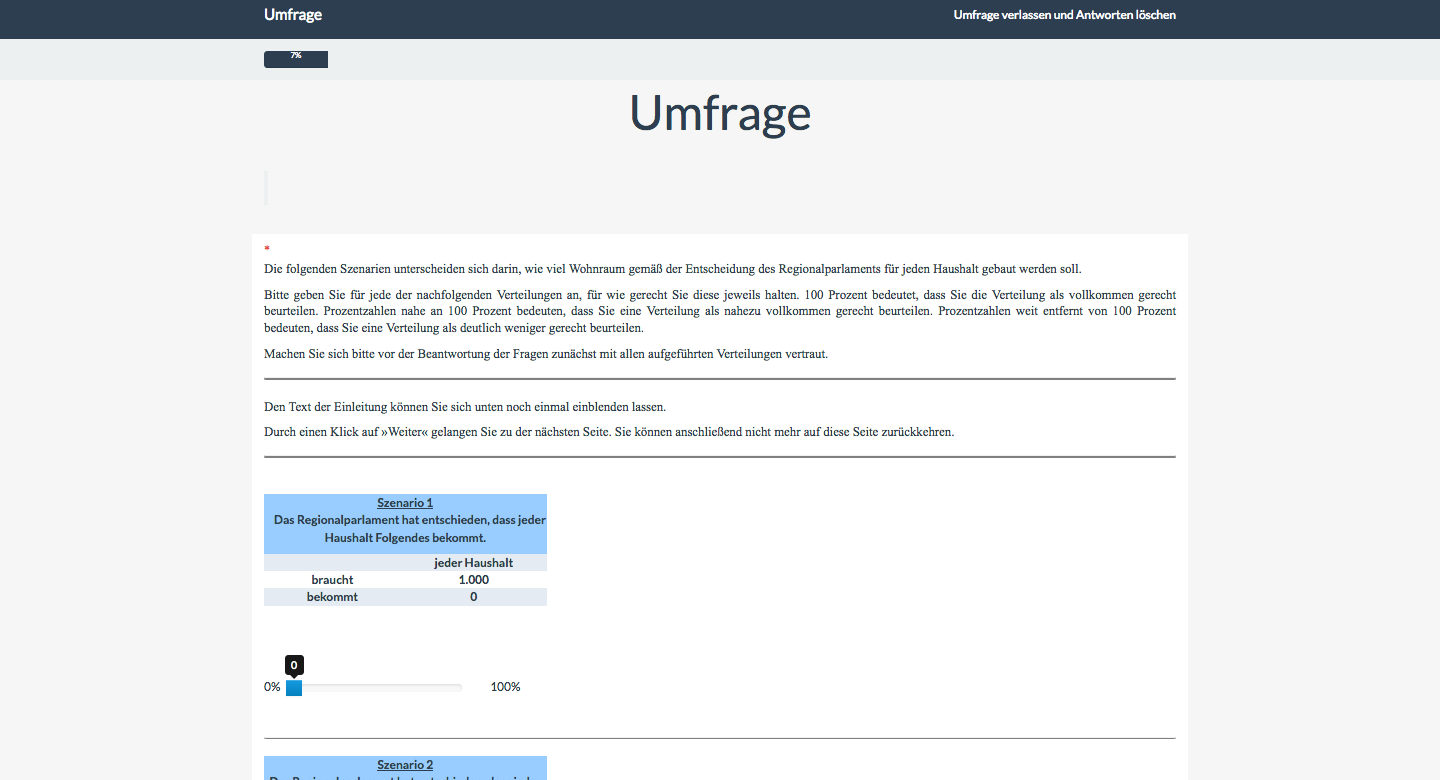
\includegraphics[width=0.5\linewidth]{figures/slides_lime_1.png}}\\
   \textcolor{gray}{Global Evaluation Task}
\end{center}
\note{
   \begin{itemize}
      \item Vignette is repeated at the top of the screen
      \item Below are tables for all cases, showing how much the households receive and how much they need
      \item Cases reach from $0$ to $2000$ units in steps of $200$
      \item Justice evaluations are entered using a slider ranging from $1$ to $100$ percent
   \end{itemize}
}
\end{frame}


%%%%%%%%%%%%
% SLIDE 11 %
%%%%%%%%%%%%
\begin{frame}{\vspace*{10mm}1\hspace*{1em}Need as Reference Point}
\textbf{Task (2/2)}\\
\begin{multicols}{2}
   \begin{center}
      \frame{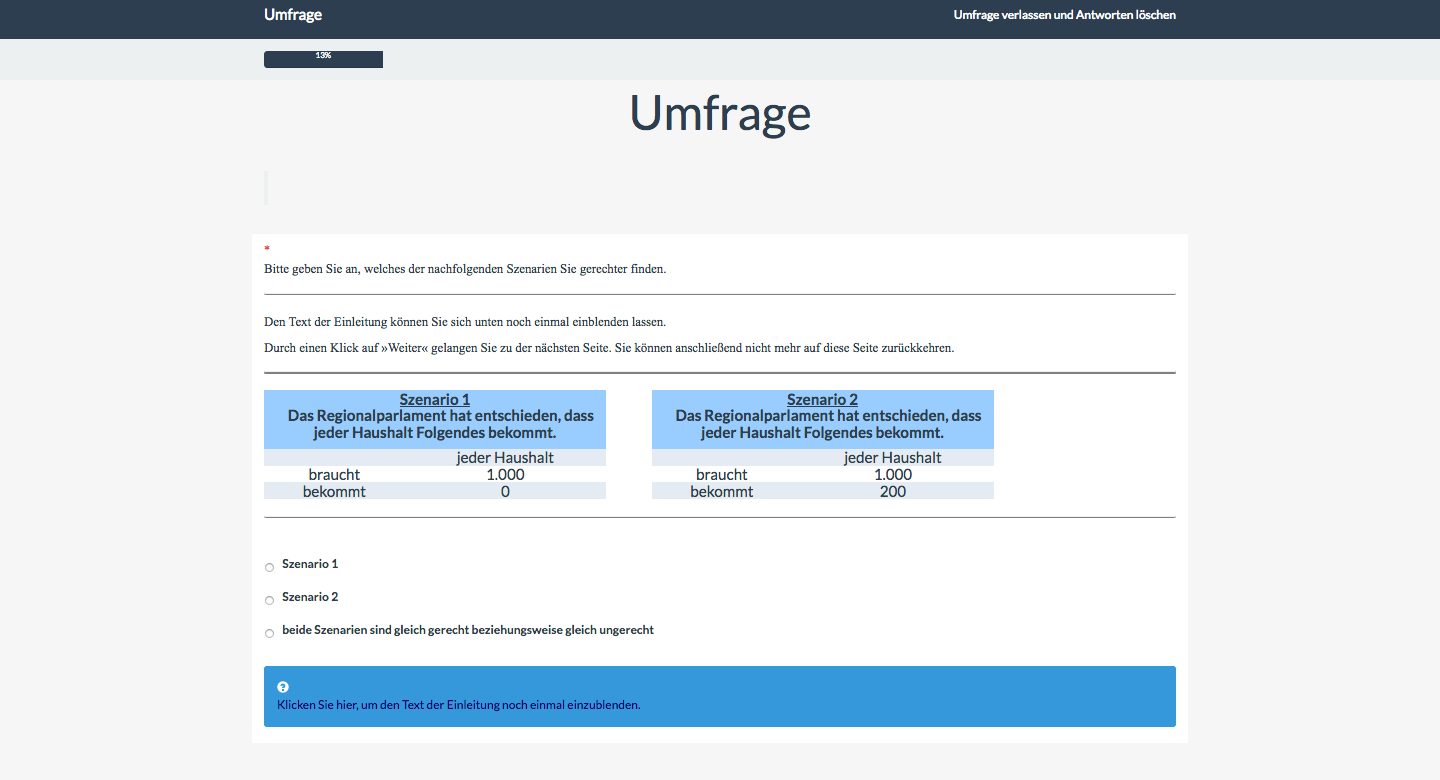
\includegraphics[width=1\linewidth]{figures/slides_lime_2.png}}\\
      \textcolor{gray}{Relative Evaluation Task (Part 1)}
      \frame{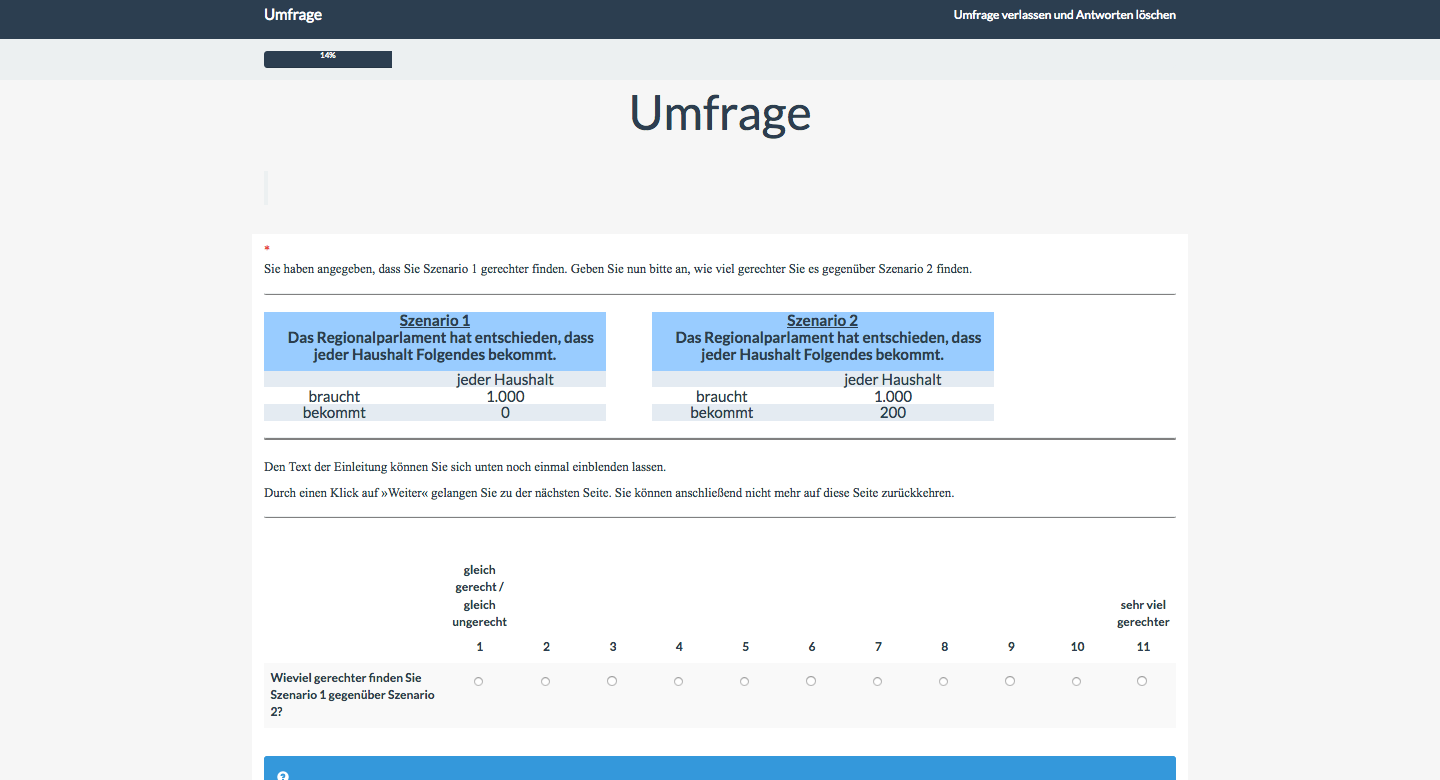
\includegraphics[width=1\linewidth]{figures/slides_lime_3.png}}\\
      \textcolor{gray}{Relative Evaluation Task (Part 2)}
   \end{center}
\end{multicols}
\note{
   \begin{itemize}
      \item $10$ pairs of adjacent cases on separate screens
      \item Participants have to decide whether one of the two is more just, and if so, which one
      \item They are then asked to indicate how much so on a scale from $1$ to $11$
   \end{itemize}
}
\end{frame}


%%%%%%%%%%%%
% SLIDE 12 %
%%%%%%%%%%%%
\begin{frame}{\vspace*{10mm}1\hspace*{1em}Need as Reference Point}
\textbf{Results (1/2)}\\
\begin{multicols}{2}
   \begin{center}
      \frame{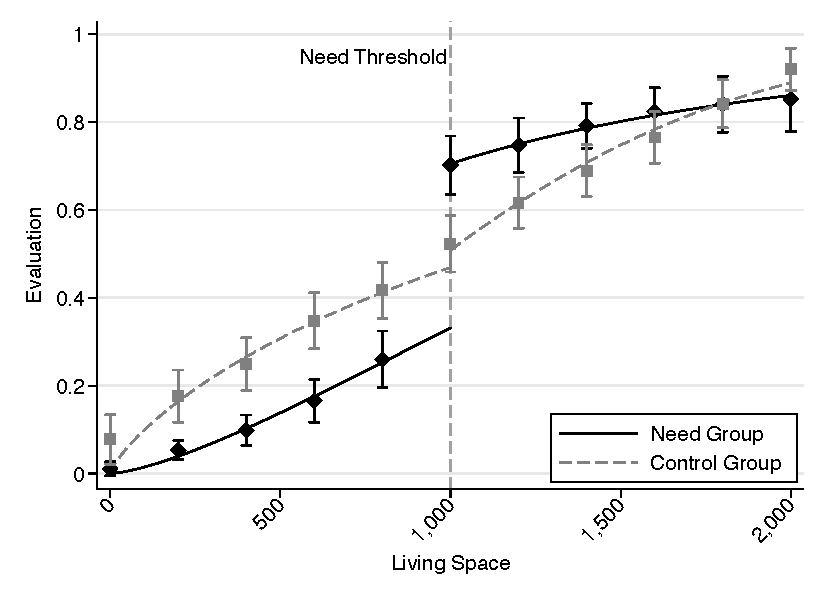
\includegraphics[width=1\linewidth]{figures/figure_1_english.pdf}}\\
      \textcolor{gray}{Global Evaluation Task}
      \frame{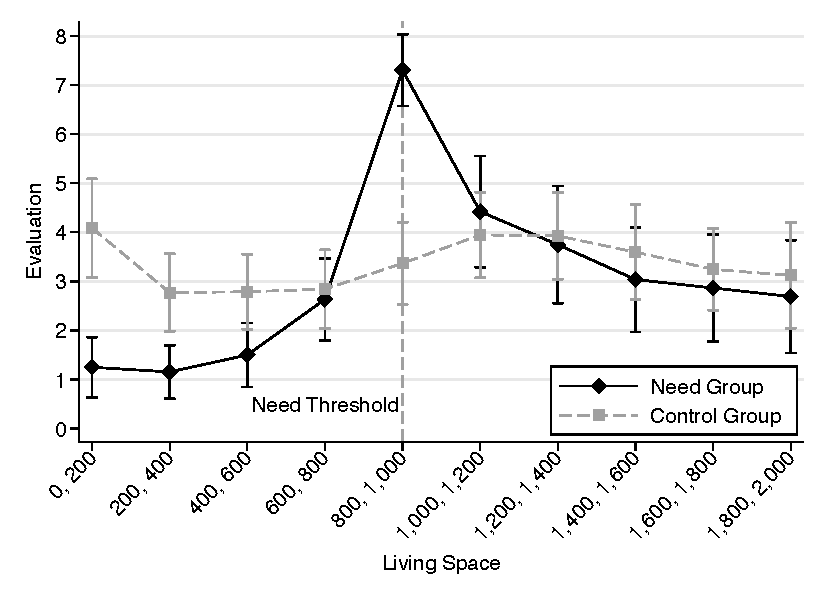
\includegraphics[width=1\linewidth]{figures/figure_2_english.pdf}}\\
      \textcolor{gray}{Relative Evaluation Task}
   \end{center}
\end{multicols}
\note{
   \begin{itemize}
      \item Global Evaluation Task
      \begin{itemize}
         \item Weibul estimation (reference points at $0$ and $1000$ units)
         \item Sharp increase (approximately $35$ percentage points), convex below the threshold, concave above
         \item Evaluations below the threshold (excluding $0$ units) significantly lower in the Need Group (Welch tests)
         \item Evaluations above the threshold (excluding $1600$, $1800$, and $2000$ units) significantly higher in the Need Group (Welch tests)
      \end{itemize}
      \item Relative Evaluation Task
      \begin{itemize}
         \item Comparisons in the Control Group fluctuate around $3$ to $4$ points
         \item Evaluations below the threshold (excluding $600$ and $800$ units) significantly lower in the Need Group (Welch tests)
         \item Evaluations at the threshold significantly higher in the Need Group (Welch tests)
      \end{itemize}
   \end{itemize}
}
\end{frame}


%%%%%%%%%%%%
% SLIDE 13 %
%%%%%%%%%%%%
\begin{frame}{\vspace*{10mm}1\hspace*{1em}Need as Reference Point}
\textbf{Results (2/2)}\\
\medskip
\begin{itemize}
   \item Impartial observers make gradual justice evaluations
   \item Evaluations depend on supply situations
   \item Evaluations are influenced by information on need
\end{itemize}
\end{frame}


%%%%%%%%%%%%%%%%%%%%%%%%%%%%%%%%%%%%%%
% SLIDE 14 – NEED AND ACCOUNTABILITY %
%%%%%%%%%%%%%%%%%%%%%%%%%%%%%%%%%%%%%%
\begin{frame}
\begin{overlayarea}{\textwidth}{0.81\paperheight}{
   \vspace*{11mm}
   \usebeamerfont{title}\textcolor{uolblue}
   {2\hspace*{1em}Need and Accountability}
}
\end{overlayarea}
\end{frame}


%%%%%%%%%%%%
% SLIDE 15 %
%%%%%%%%%%%%
\begin{frame}{\vspace*{10mm}2\hspace*{1em}Need and Accountability}
\begin{multicols}{2}
   \textbf{Background}\\
   \medskip
   \begin{itemize}
      \item Distribution decisions reveal distributional preferences
      \item People take various (normatively relevant) factors into account when making distribution decisions
      \item What role do differences in productivity, need, and accountability play in impartial distribution decisions?
   \end{itemize}
   \vfill
   \begin{center}
      \frame{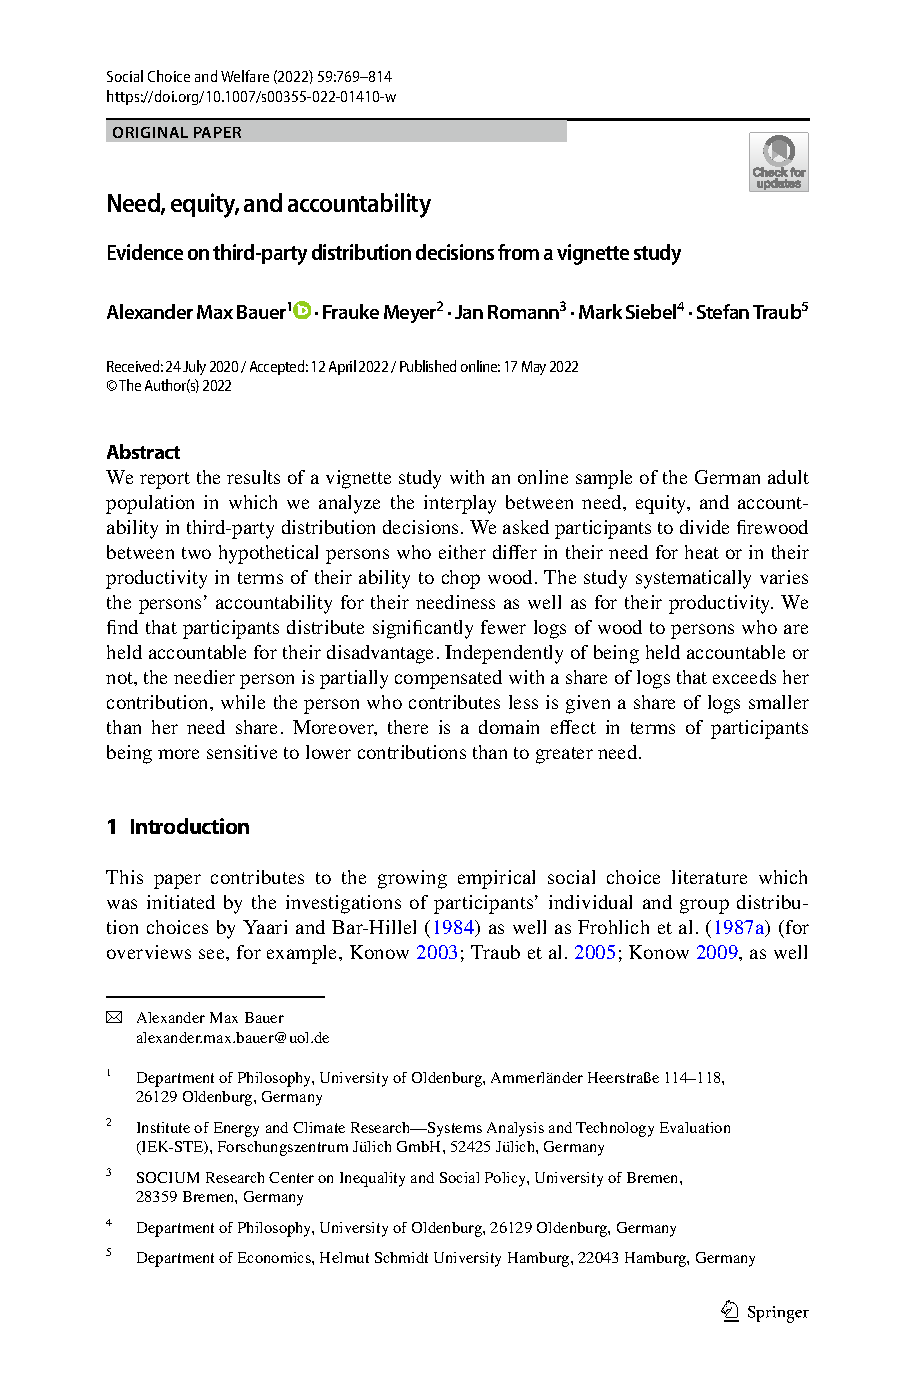
\includegraphics[width=0.6\linewidth]{figures/slides_bauer_et_al_2022.pdf}}\\
      \textcolor{gray}{Bauer et al. 2022}
   \end{center}
\end{multicols}
\end{frame}


%%%%%%%%%%%%
% SLIDE 16 %
%%%%%%%%%%%%
\begin{frame}{\vspace*{10mm}2\hspace*{1em}Need and Accountability}
\textbf{Design and Implementation (1/2)}\\
\medskip
\begin{itemize}
   \item Respondi, online panel, September 2019
   \item $n=200$ (stratified by gender, age, and net equivalent household income)
   \item Impartial decision-makers
   \item High and Low Accountability Group (\textit{between subjects})
   \item Need and Productivity Scenario (\textit{within subjects})
   \item $10$ cases
\end{itemize}
\end{frame}


%%%%%%%%%%%%
% SLIDE 17 %
%%%%%%%%%%%%
\begin{frame}{\vspace*{10mm}2\hspace*{1em}Need and Accountability}
\textbf{Vignette (High Responsibility Treatment, Productivity Scenario)}\\
\medskip
\enquote{Please imagine two persons, A and B, who do not know each other.
Both heat their huts exclusively with firewood and have enough logs in stock to survive in winter.
However, they need additional firewood in order not to feel cold in winter.
The community allows the two persons to chop wood in the community forest for a certain period of time.
A and B have little money and therefore have no other way to get firewood.\\
\medskip
A and B both need $x$ logs.
If they get less than they need, it will get unreasonably cold in their huts.
The less firewood they get, the colder their huts will be.
The persons can use more firewood than they need to heat their huts up to pleasant temperatures or store it for subsequent winters.\\
\medskip
A has chopped $y$ logs and B has chopped $z$ logs.\\
\medskip
A continued to smoke heavily against the advice of their doctor and is suffering from a cardiovascular disease.
That is why A has chopped less wood than B.}
\note{
   \begin{itemize}
      \item Here and in the following: if a variable represents a name, the name was randomly drawn from a pool of common German surnames
      \item \enquote{A suffers from a congenital cardiovascular disease. Therefore, A chopped less wood than B.}
      \item \enquote{A suffers from a congenital metabolic disease, which is why they need a higher room temperature. Therefore, A needs more firewood than B.}
   \end{itemize}
}
\end{frame}


%%%%%%%%%%%%
% SLIDE 18 %
%%%%%%%%%%%%
\begin{frame}{\vspace*{10mm}2\hspace*{1em}Need and Accountability}
\textbf{Design and Implementation (2/2)}\\
\medskip
\begin{center}
   \begin{tabular}{lrrrrr}
      \arrayrulecolor{blue2}
      \hline
      Case                      & \multicolumn{1}{c}{1}     & \multicolumn{1}{c}{2}     & \multicolumn{1}{c}{3}     & \multicolumn{1}{c}{4}     & \multicolumn{1}{c}{5}     \\
      \hline\hline\\[-0.5em]
                                & \multicolumn{5}{c}{Need Scenario}                                                                                                         \\[0.5em]
      Need A                    &                  1.800    &                  1.400    &                  1.000    &                    700    &                    600    \\
      Productivity A            & \textcolor{gray}{1.000}   & \textcolor{gray}{1.000}   & \textcolor{gray}{1.000}   & \textcolor{gray}{1.000}   & \textcolor{gray}{1.000}   \\[0.5em]
      Need B                    &                  1.200    &                    800    &                    400    &                    200    &                    100    \\
      Productivity B            & \textcolor{gray}{1.000}   & \textcolor{gray}{1.000}   & \textcolor{gray}{1.000}   & \textcolor{gray}{1.000}   & \textcolor{gray}{1.000}   \\
      \hline
                                & \multicolumn{5}{c}{Productivity Scenario}                                                                                                 \\[0.5em]
      Need A                    & \textcolor{gray}{1.000}   & \textcolor{gray}{1.000}   & \textcolor{gray}{1.000}   & \textcolor{gray}{1.000}   & \textcolor{gray}{1.000}   \\
      Productivity A            &                  1.200    &                    800    &                    400    &                    200    &                    100    \\[0.5em]
      Need B                    & \textcolor{gray}{1.000}   & \textcolor{gray}{1.000}   & \textcolor{gray}{1.000}   & \textcolor{gray}{1.000}   & \textcolor{gray}{1.000}   \\
      Productivity B            &                  1.800    &                  1.400    &                  1.000    &                    700    &                    600    \\
      \hline
   \end{tabular}\\
   \smallskip
   \textcolor{gray}{Parameterization}
\end{center}
\note{
   \begin{itemize}
      \item Heterogeneities as justifications for inequalities in distribution
      \item Person A always worse-off
      \item In High Accountability Treatment: Person A accountable for their greater need or lower productivity
   \end{itemize}
}
\end{frame}


%%%%%%%%%%%%
% SLIDE 19 %
%%%%%%%%%%%%
\begin{frame}{\vspace*{10mm}2\hspace*{1em}Need and Accountability}
\textbf{Task}\\
\medskip
\begin{center}
   \frame{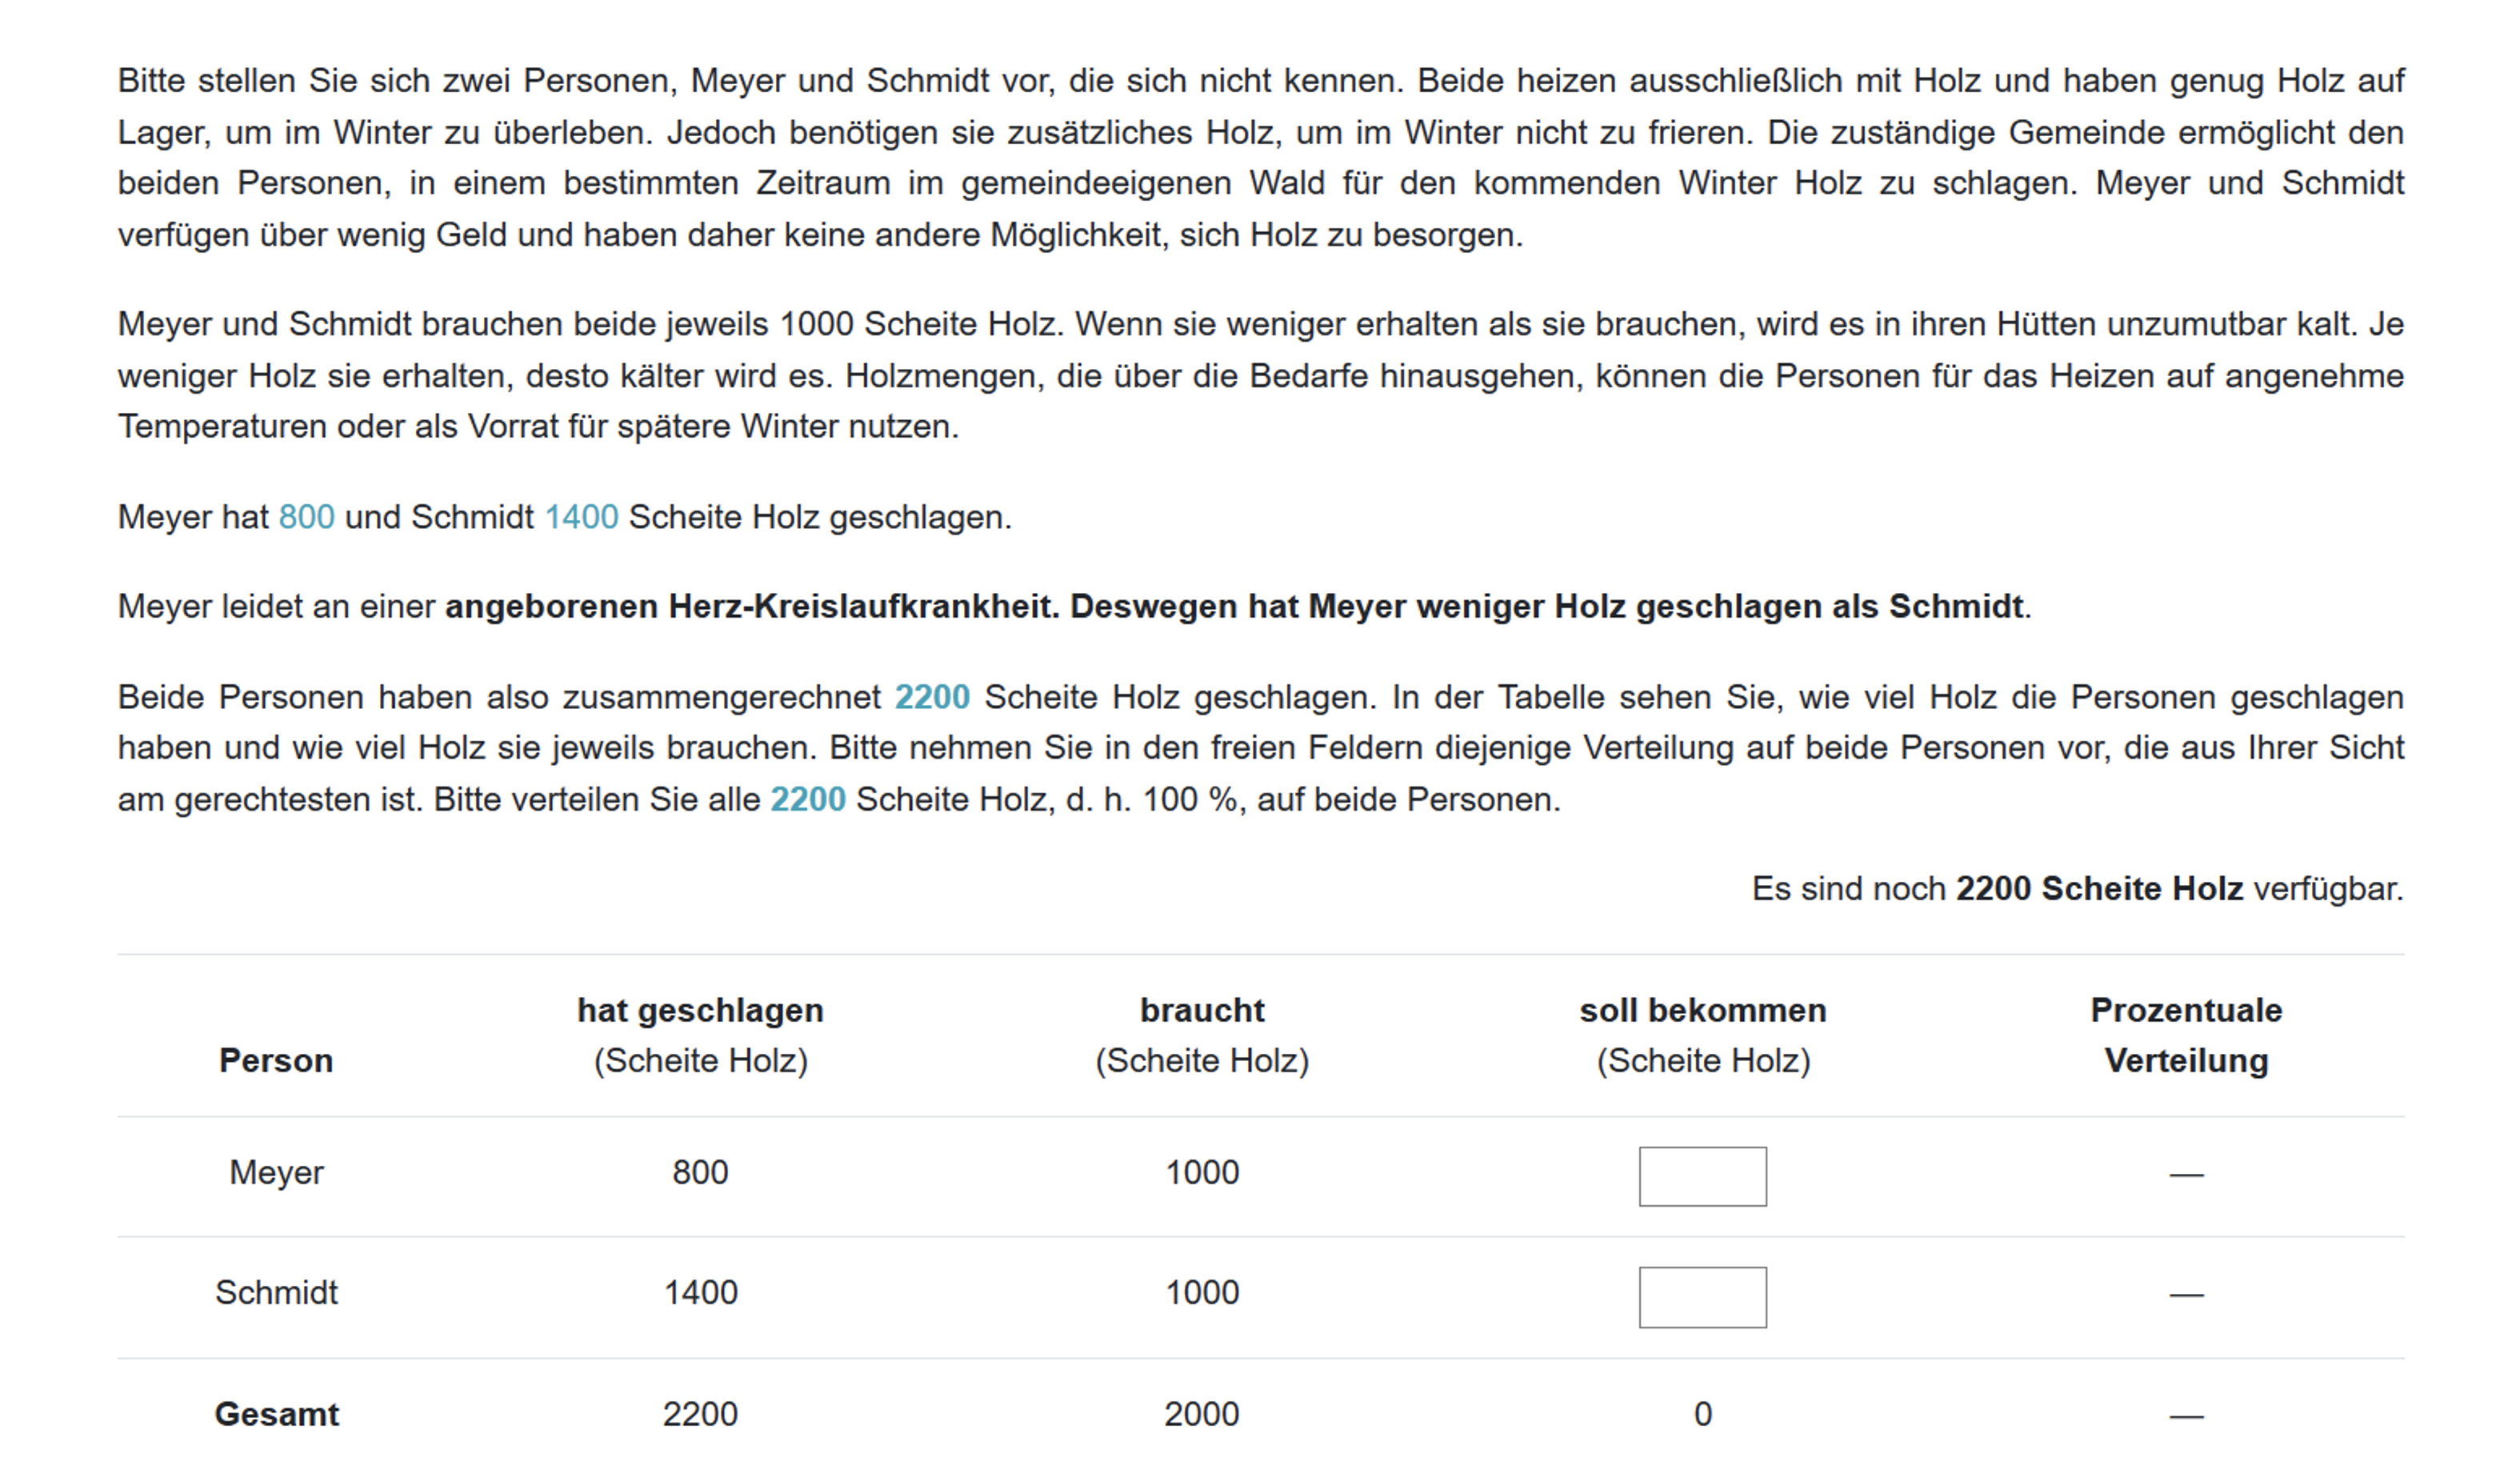
\includegraphics[width=0.5\linewidth]{figures/slides_otree_1.png}}\\
   \textcolor{gray}{Distribution Task\\(Low Responsibility Treatment, Productivity Scenario)}
\end{center}
\note{
   \begin{itemize}
      \item Vignette is repeated at the top of the screen
      \item Below is a table showing how much each person has produced and how much they need
      \item Two fields where subjects could enter how much each person should receive
   \end{itemize}
}
\end{frame}


%%%%%%%%%%%%
% SLIDE 20 %
%%%%%%%%%%%%
\begin{frame}{\vspace*{10mm}2\hspace*{1em}Need and Accountability}
\textbf{Results (1/3)}\\
\medskip
\begin{center}
   Share of Logs $=\frac{\gamma_{A}}{\Gamma}$
\end{center}
\note{
   \begin{itemize}
      \item Normalized share of logs, since the available amount is not identical over all cases
      \item Additionally: normalized deviation from equal split
   \end{itemize}
}
\end{frame}


%%%%%%%%%%%%
% SLIDE 21 %
%%%%%%%%%%%%
\begin{frame}{\vspace*{10mm}2\hspace*{1em}Need and Accountability}
\textbf{Results (2/3)}\\
\medskip
\begin{center}
   \frame{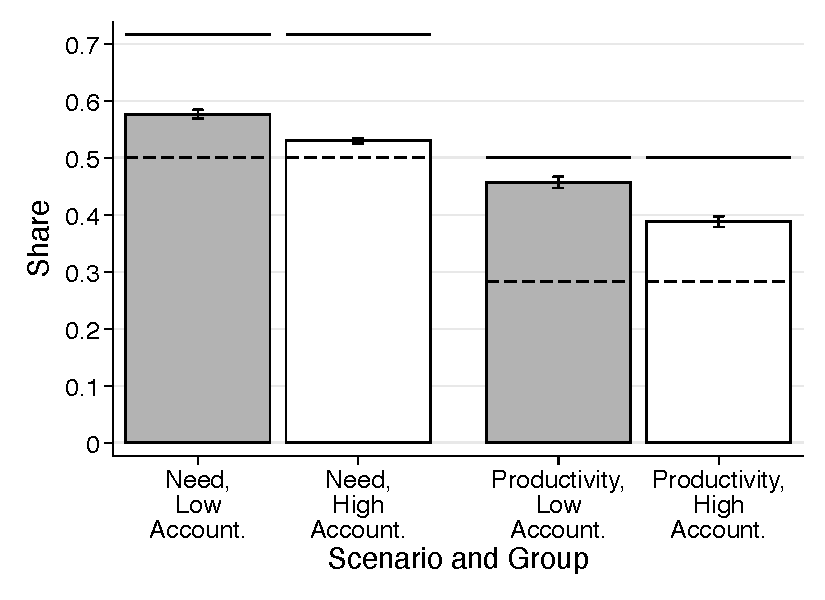
\includegraphics[width=0.5\linewidth]{figures/figure_7_a_english.pdf}}\\
   \textcolor{gray}{Share of Logs}
\end{center}
\note{
   \begin{itemize}
      \item $2.000$ distribution decisions ($10\times200$)
      \item Solid line: Person A's need share
      \item Dashed line: Person A's productivity share
      \item Higher than the productivity share and lower than the need share (one-sided $t$-tests)
      \item Lower when accountable (one-sided $t$-tests)
      \item Additionally: GLS panel regressions
   \end{itemize}
}
\end{frame}


%%%%%%%%%%%%
% SLIDE 22 %
%%%%%%%%%%%%
\begin{frame}{\vspace*{10mm}2\hspace*{1em}Need and Accountability}
\textbf{Results (3/3)}\\
\medskip
\begin{itemize}
   \item Impartial decision-makers take need, productivity, and accountability into account
   \item Even in cases of low productivity, need is partially compensated
   \item Willingness to compensate decreases when low productivity or high need is self-inflicted
\end{itemize}
\end{frame}


%%%%%%%%%%%%
% SLIDE 23 %
%%%%%%%%%%%%
\begin{frame}{\vspace*{10mm}2\hspace*{1em}Need and Accountability}
\begin{multicols}{2}
   \textbf{Replication}\\
   \medskip
   \begin{itemize}
      \item Respondi, online panel, November 2020
      \item $n=400$ (stratified as above)
      \item High and Low Accountability Group (\textit{within subject})
      \item Oversupply and Undersupply Scenario (\textit{within subject})
      \item $10$ (different) cases
   \end{itemize}
   \vfill
   \begin{center}
      \frame{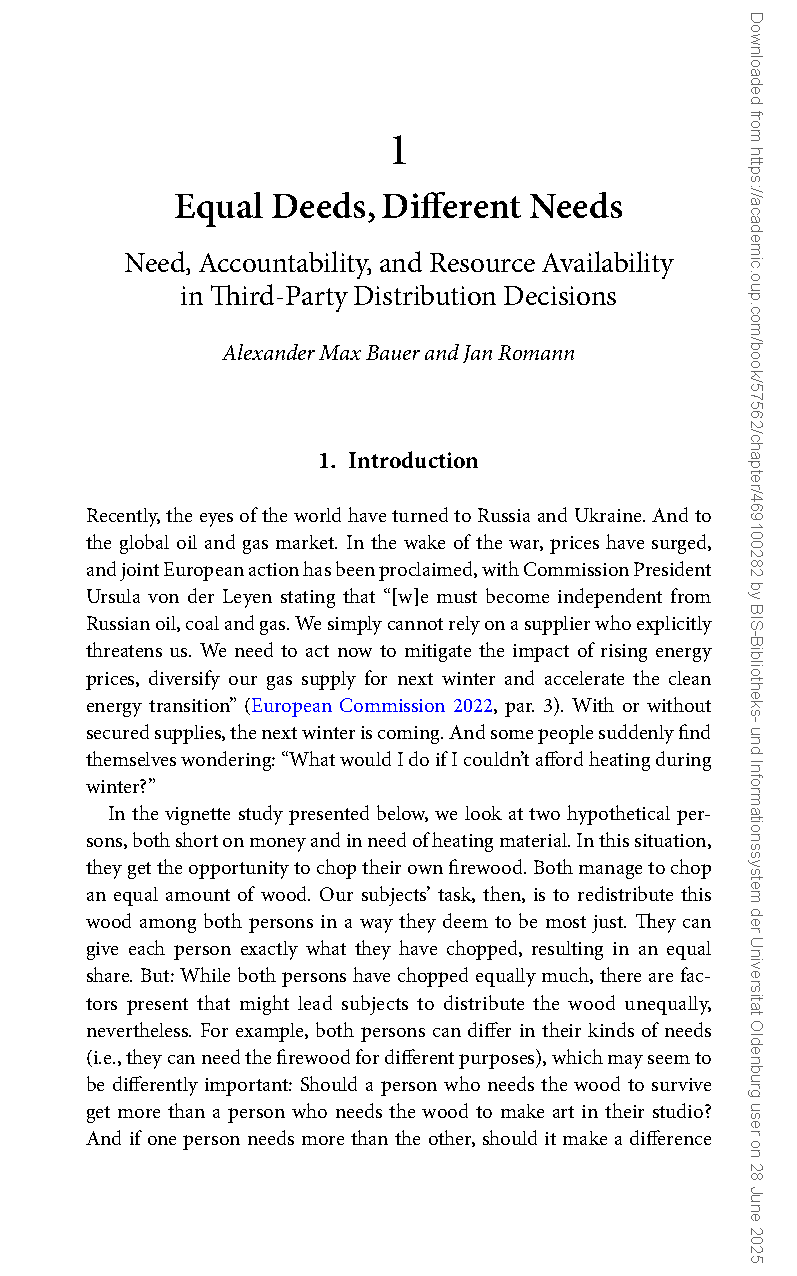
\includegraphics[width=0.5\linewidth]{figures/slides_bauer_romann_2024.pdf}}\\
      \textcolor{gray}{Bauer and Romann 2024}
   \end{center}
\end{multicols}
\end{frame}


%%%%%%%%%%%%%%%%%%%%%%%%%%%%%
% SLIDE 24 – KINDS OF NEEDS %
%%%%%%%%%%%%%%%%%%%%%%%%%%%%%
\begin{frame}
\begin{overlayarea}{\textwidth}{0.81\paperheight}{
   \vspace*{11mm}
   \usebeamerfont{title}\textcolor{uolblue}
   {3\hspace*{1em}Kinds of Needs}
}
\end{overlayarea}
\end{frame}


%%%%%%%%%%%%
% SLIDE 25 %
%%%%%%%%%%%%
\begin{frame}{\vspace*{10mm}3\hspace*{1em}Kinds of Needs}
\begin{multicols}{2}
   \textbf{Background}\\
   \medskip
   \begin{itemize}
      \item Philosophical and psychological literature distinguishes between different kinds of needs
      \item What role do different kinds of needs play for impartial observers (Study 1) and decision-makers (Study 2)?
   \end{itemize}
   \vfill
   \begin{center}
      \frame{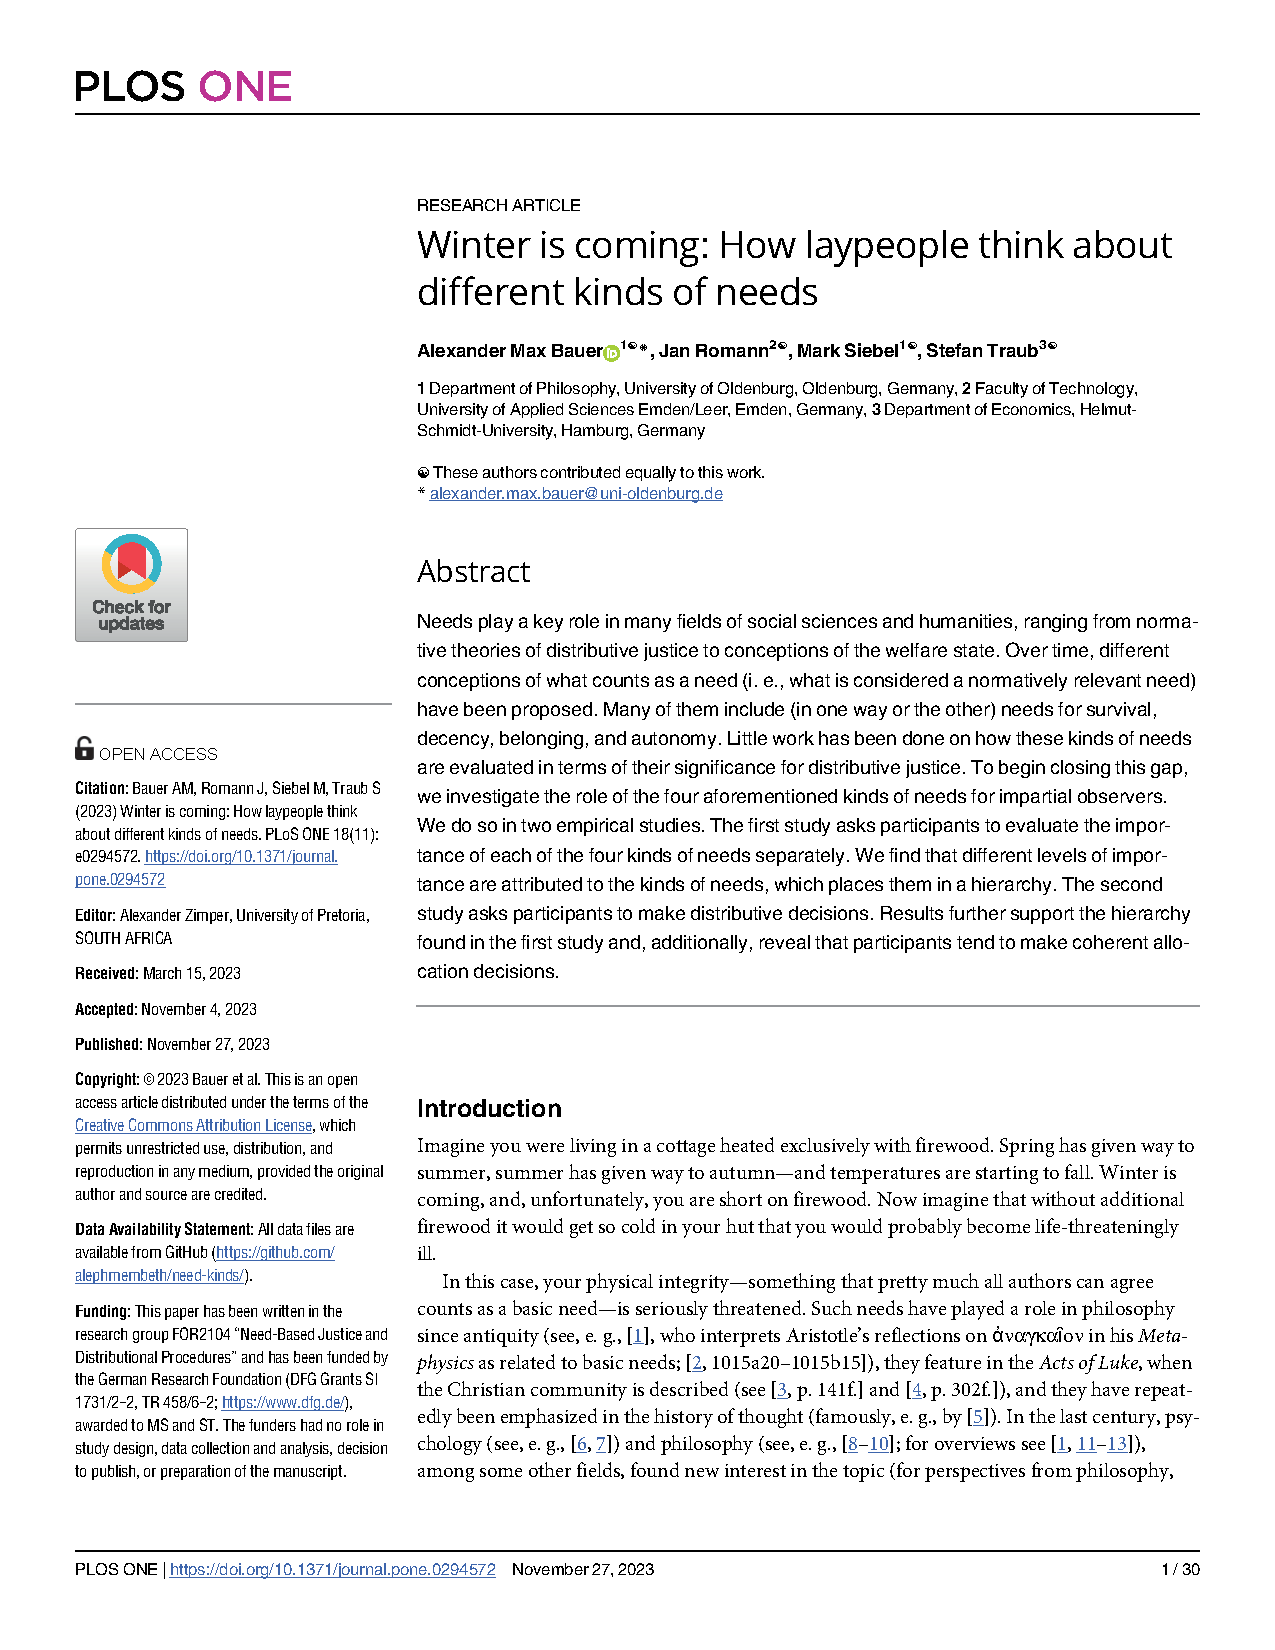
\includegraphics[width=0.6\linewidth]{figures/slides_bauer_et_al_2023b.pdf}}\\
      \textcolor{gray}{Bauer et al. 2023}
   \end{center}
\end{multicols}
\end{frame}


%%%%%%%%%%%%%%%%%%%%%
% SLIDE 26 – STUDY 1%
%%%%%%%%%%%%%%%%%%%%%
\begin{frame}
\begin{overlayarea}{\textwidth}{0.81\paperheight}{
   \vspace*{11mm}
   \usebeamerfont{title}\textcolor{uolblue}
   {3.1\hspace*{1em}Study 1}
}
\end{overlayarea}
\end{frame}


%%%%%%%%%%%%
% SLIDE 27 %
%%%%%%%%%%%%
\begin{frame}{\vspace*{10mm}3.1\hspace*{1em}Study 1}
\textbf{Design and Implementation}\\
\medskip
\begin{itemize}
   \item Respondi, online panel, February 2021
   \item $n=100$ (stratified as above)
   \item Impartial observers
   \item $4$ kinds of needs (\textit{within subjects})
   \item $4$ cases
\end{itemize}
\note{
   \begin{itemize}
      \item Randomized overview of the $4$ kinds of needs
      \item Presentation on four separate screens in the same order for evaluation
   \end{itemize}
}
\end{frame}


%%%%%%%%%%%%
% SLIDE 28 %
%%%%%%%%%%%%
\begin{frame}{\vspace*{10mm}3.1\hspace*{1em}Study 1}
\textbf{Vignette (1/5)}\\
\medskip
\enquote{Please imagine four people with the names A, B, C, and D.
All are in need for wood.
They need the wood for different reasons.
On this page, we present to you the different reasons for which A, B, C, and D need the wood.
On the following pages, you will be asked how important it is that the respective person's need is met.}
\end{frame}


%%%%%%%%%%%%
% SLIDE 29 %
%%%%%%%%%%%%
\begin{frame}{\vspace*{10mm}3.1\hspace*{1em}Study 1}
\begin{multicols}{2}
   \textbf{Vignette (2/5)}\\
   \medskip
   \enquote{A needs the wood to make sure to survive the coming winter.
   If A receives less than he needs, it will be so cold in his hut that he is very likely to become life-threateningly ill.
   The less wood he receives, the higher the probability that he will become life-threateningly ill.}
   \vfill
   \begin{center}
      \frame{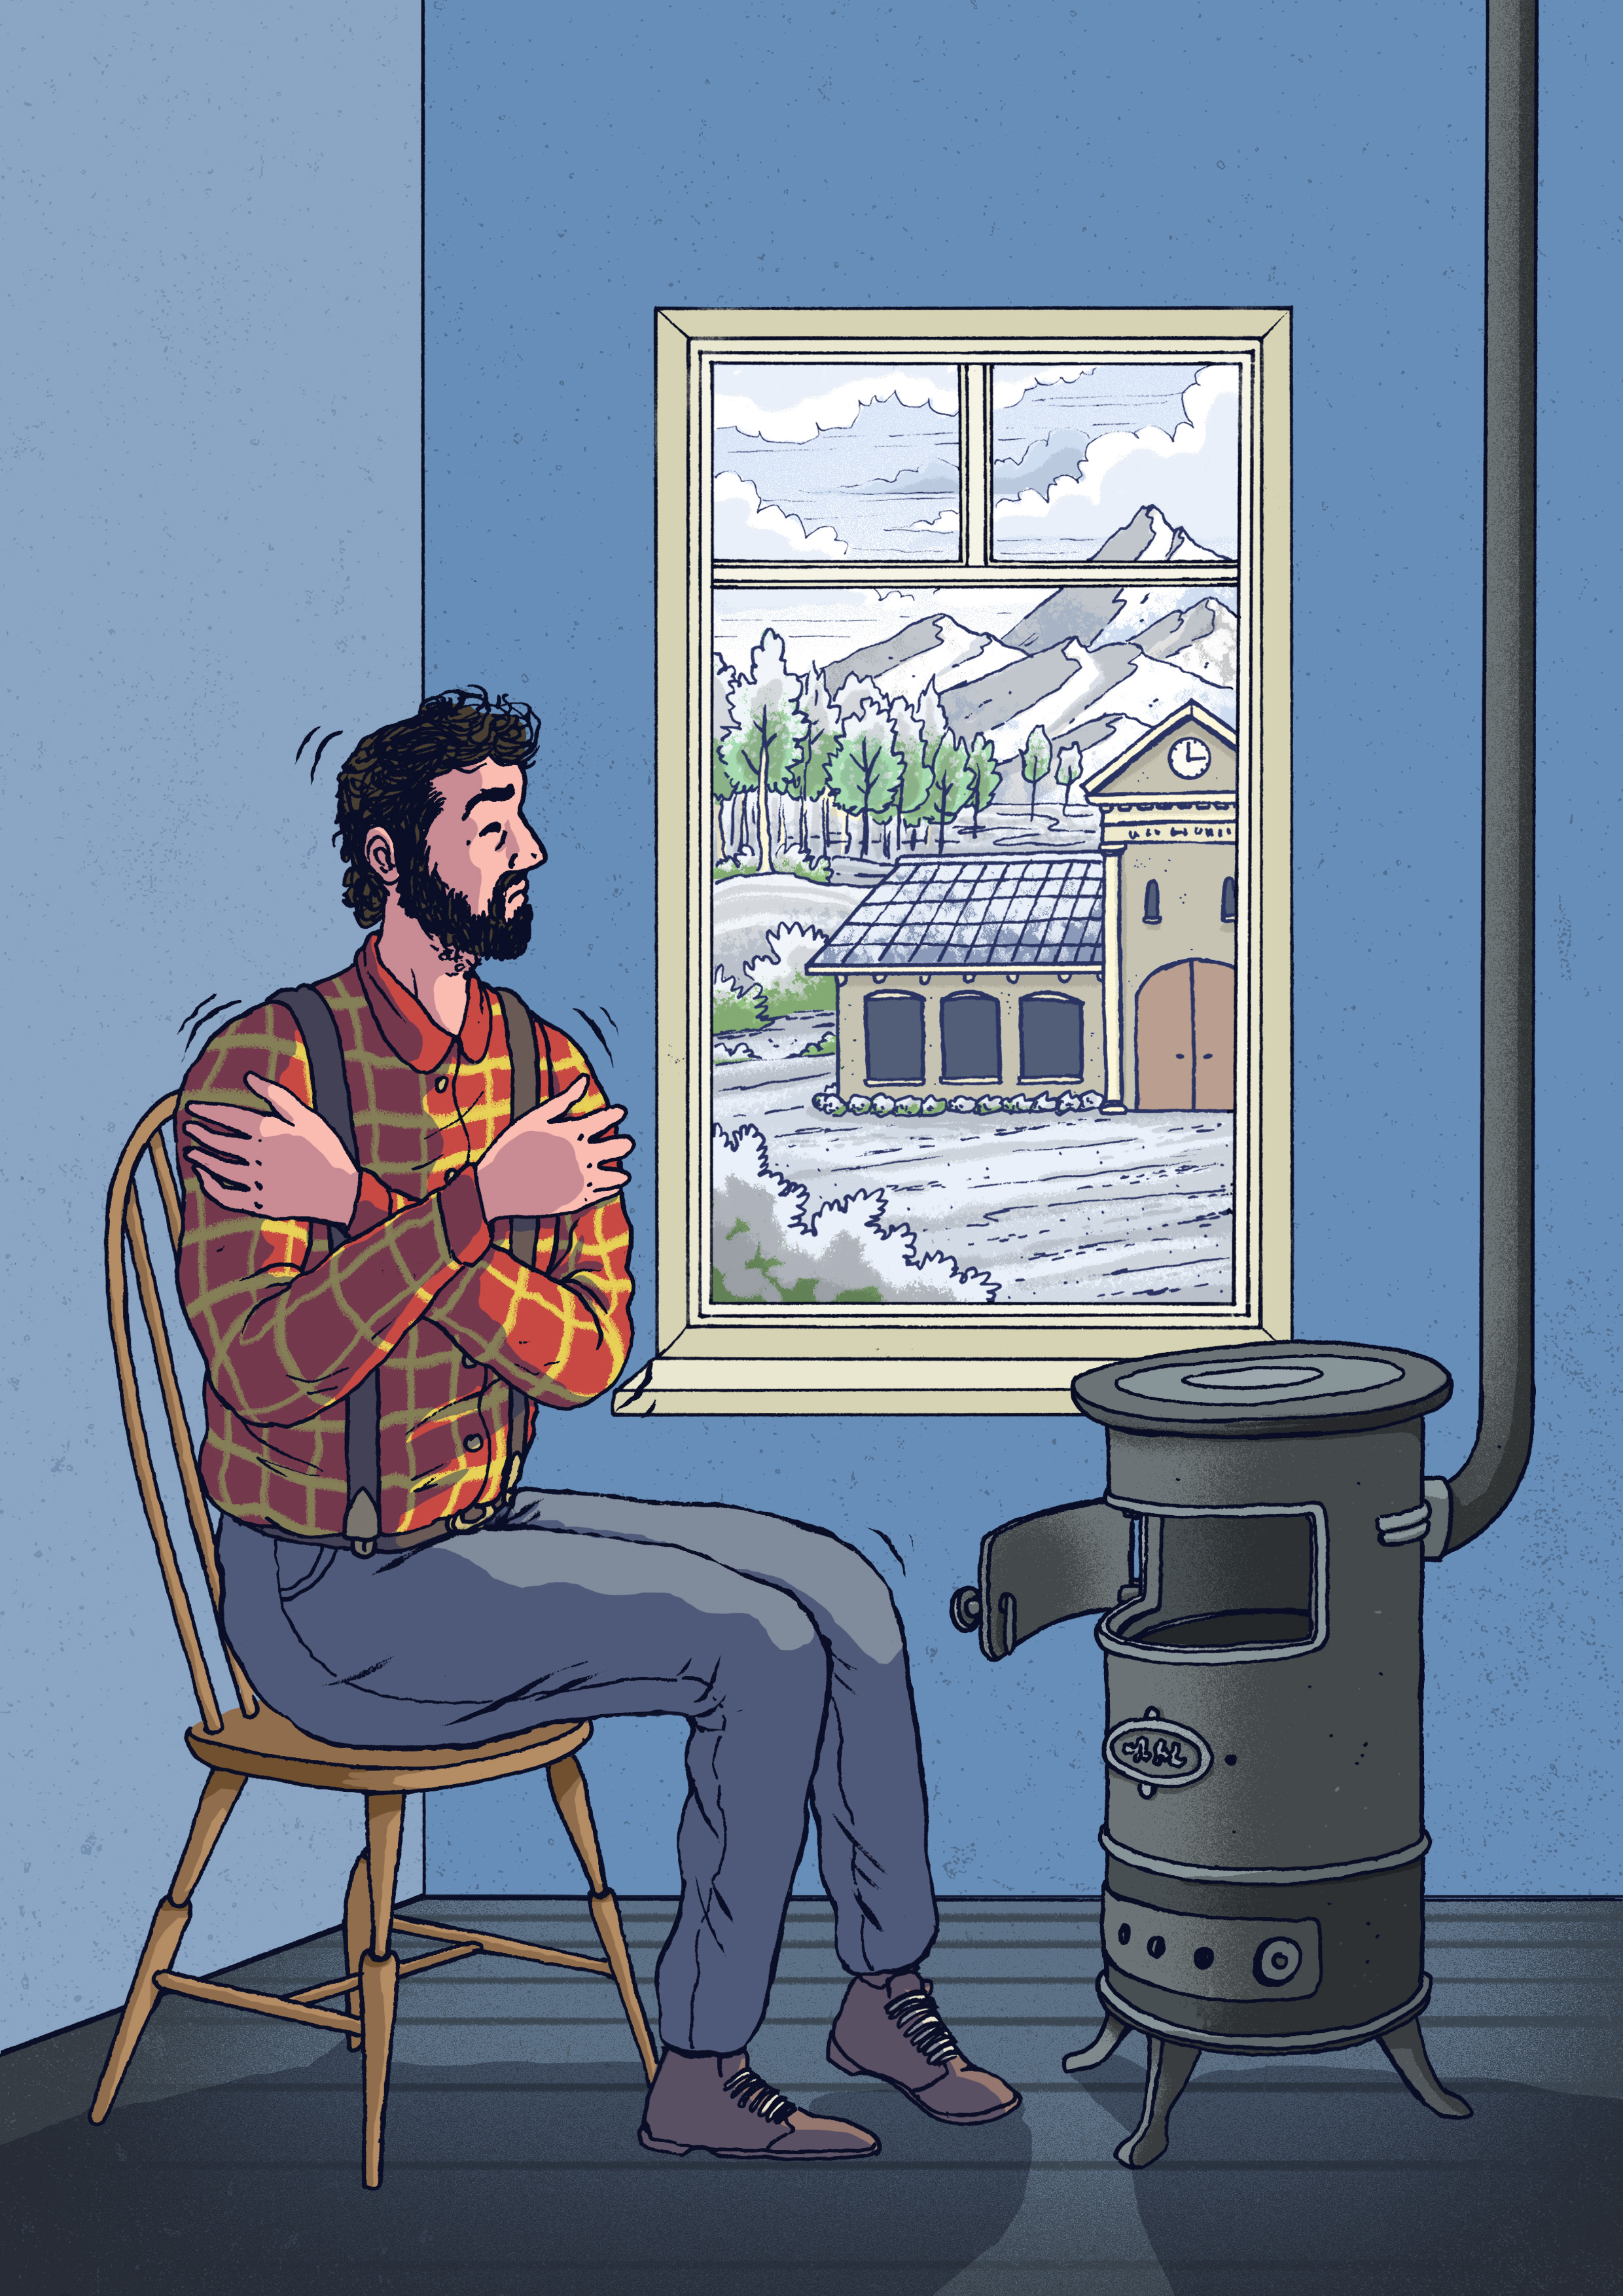
\includegraphics[width=0.6\linewidth]{figures/figure_11.jpg}}\\
      \textcolor{gray}{Illustration \textit{Survival}}
   \end{center}
\end{multicols}
\note{
   \begin{itemize}
      \item Illustrations by Douwe Dijkstra
   \end{itemize}
}
\end{frame}


%%%%%%%%%%%%
% SLIDE 30 %
%%%%%%%%%%%%
\begin{frame}{\vspace*{10mm}3.1\hspace*{1em}Study 1}
\begin{multicols}{2}
   \textbf{Vignette (3/5)}\\
   \medskip
   \enquote{B needs the wood in order not to freeze in the coming winter.
   The members of the community to which B belongs agree that one cannot live in dignity if one has to freeze.
   If B receives less than he needs, it becomes unacceptably cold in his hut.
   The less wood he receives, the more often he will freeze.}
   \vfill
   \begin{center}
      \frame{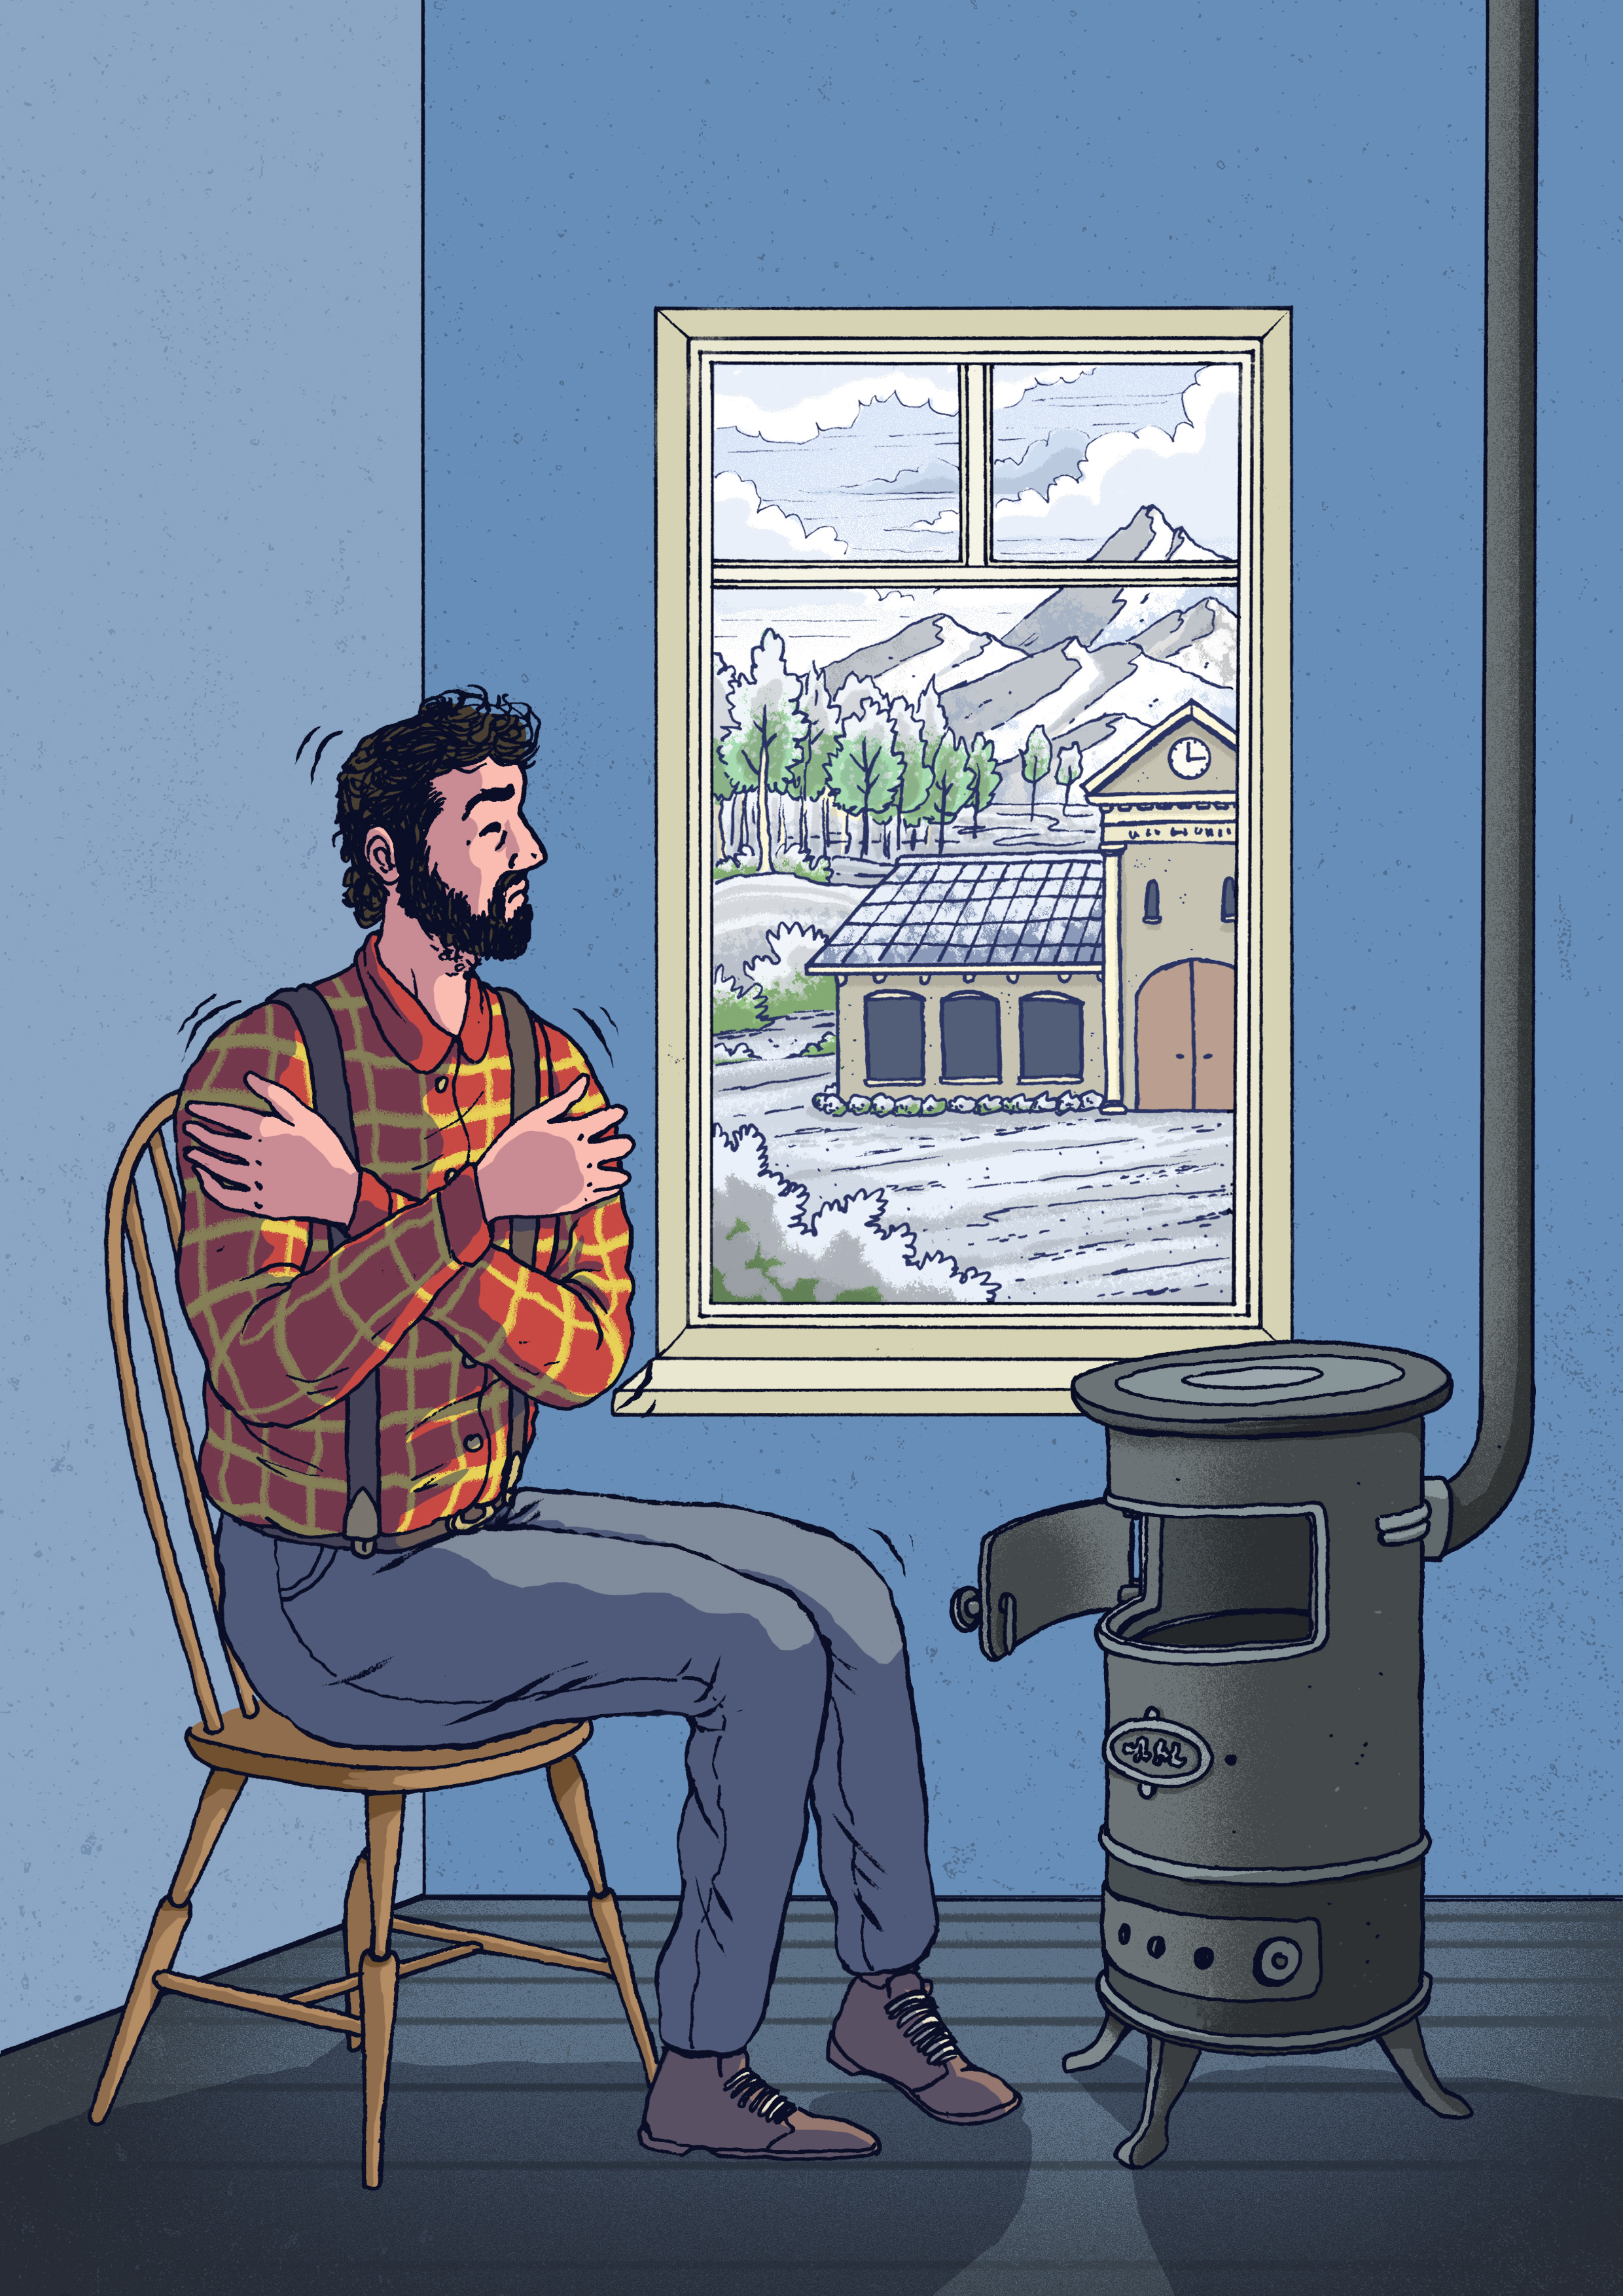
\includegraphics[width=0.6\linewidth]{figures/figure_12.jpg}}\\
      \textcolor{gray}{Illustration \textit{Decency}}
   \end{center}
\end{multicols}
\end{frame}


%%%%%%%%%%%%
% SLIDE 31 %
%%%%%%%%%%%%
\begin{frame}{\vspace*{10mm}3.1\hspace*{1em}Study 1}
\begin{multicols}{2}
   \textbf{Vignette (4/5)}\\
   \medskip
   \enquote{C needs the wood to be able to participate regularly in the social life of his community in the coming winter.
   It is common practice to meet at the community center and everyone brings wood with which to heat it.
   If C receives less than he needs, he will not be able to participate regularly in the social life.
   The less wood he receives, the less often he will be able to come to meetings at the community center.}
   \vfill
   \begin{center}
      \frame{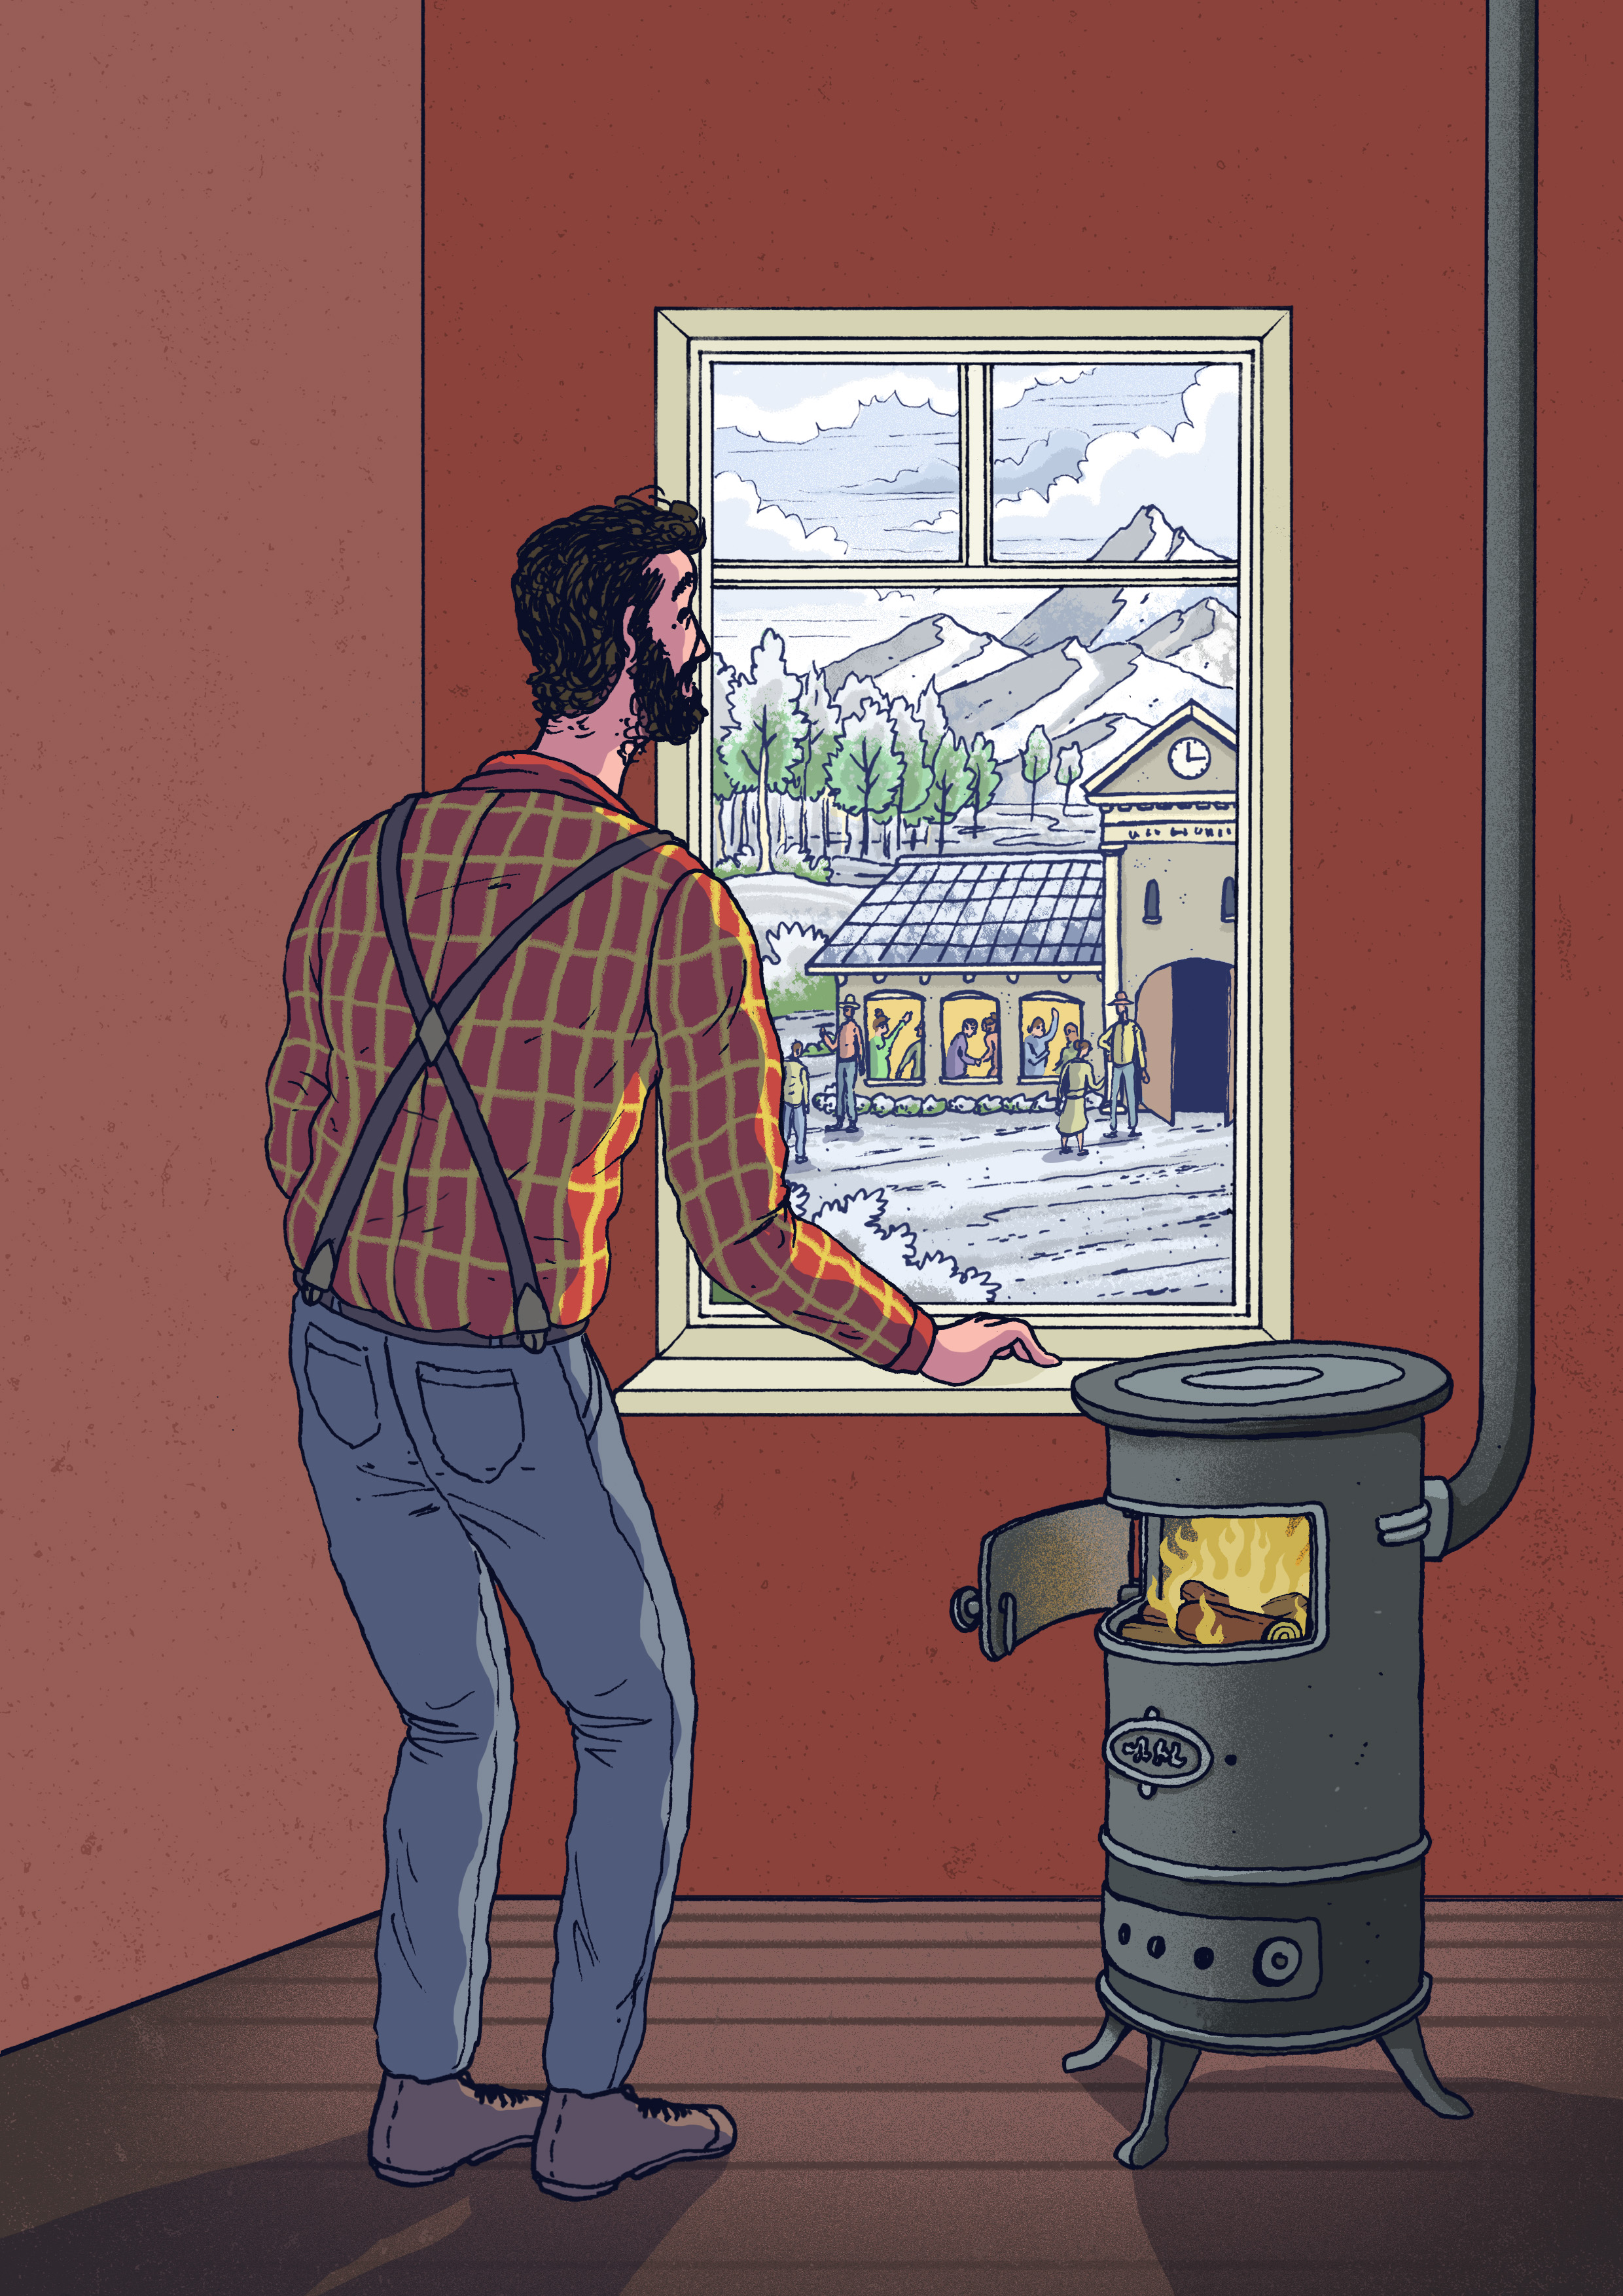
\includegraphics[width=0.6\linewidth]{figures/figure_13.jpg}}\\
      \textcolor{gray}{Illustration \textit{Belonging}}
   \end{center}
\end{multicols}
\end{frame}


%%%%%%%%%%%%
% SLIDE 32 %
%%%%%%%%%%%%
\begin{frame}{\vspace*{10mm}3.1\hspace*{1em}Study 1}
\begin{multicols}{2}
   \textbf{Vignette (5/5)}\\
   \medskip
   \enquote{D needs the wood to be able to use his studio regularly in the coming winter.
   He creates art there in his spare time.
   If D receives less than he needs, he will not be able to use his studio regularly.
   The less wood he receives, the less often he will be able to create art in his studio.}
   \vfill
   \begin{center}
      \frame{
\includegraphics[width=0.6\linewidth]{figures/figure_14.jpg}}\\
      \textcolor{gray}{Illustration \textit{Autonomy}}
   \end{center}
\end{multicols}
\end{frame}


%%%%%%%%%%%%
% SLIDE 33 %
%%%%%%%%%%%%
\begin{frame}{\vspace*{10mm}3.1\hspace*{1em}Study 1}
\textbf{Task}\\
\medskip
\begin{center}
   \frame{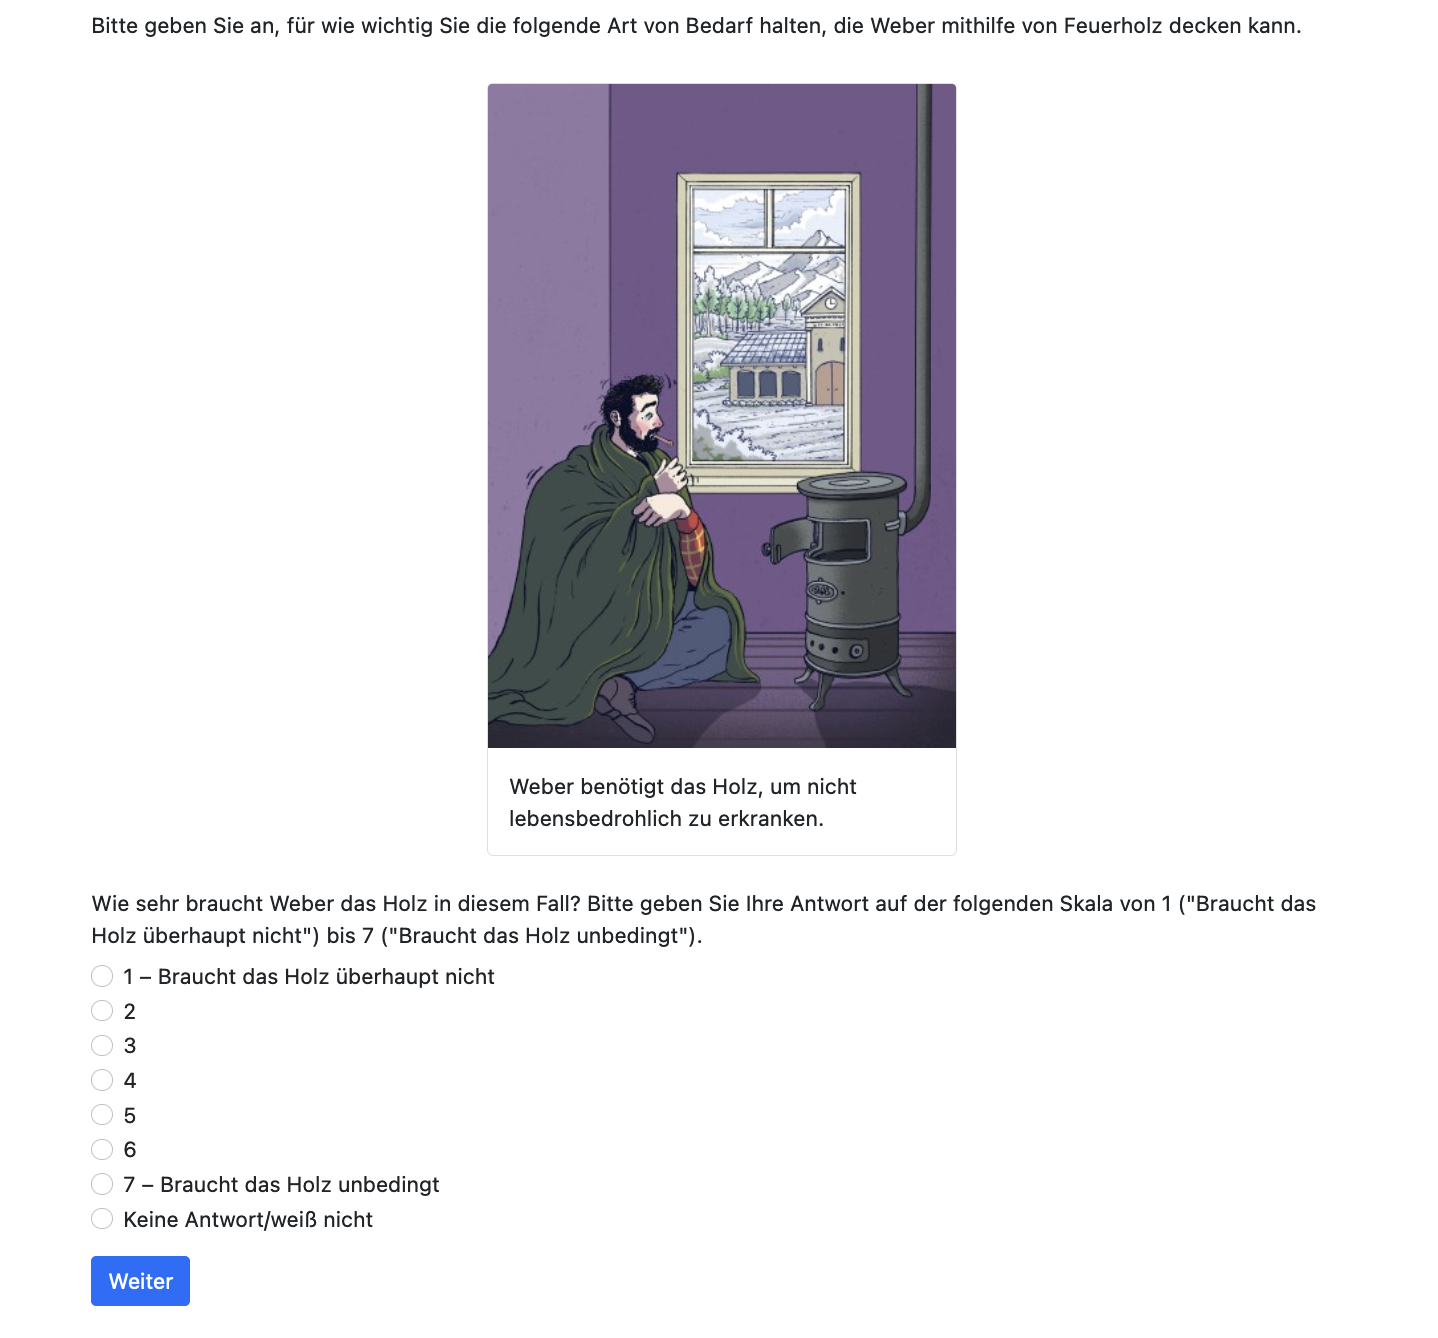
\includegraphics[width=0.4\linewidth]{figures/slides_otree_2.png}}\\
   \textcolor{gray}{Evaluation Task \textit{Survival}}
\end{center}
\note{
   \begin{itemize}
      \item Illustration is repeated at the top of the screen together with a summary sentence
      \item Below, participants could indicate on a scale from $1$ to $7$ how important they considered the fulfillment of the kind of need
   \end{itemize}
}
\end{frame}


%%%%%%%%%%%%
% SLIDE 34 %
%%%%%%%%%%%%
\begin{frame}{\vspace*{10mm}3.1\hspace*{1em}Study 1}
\textbf{Results (1/2)}\\
\medskip
\begin{center}
   \frame{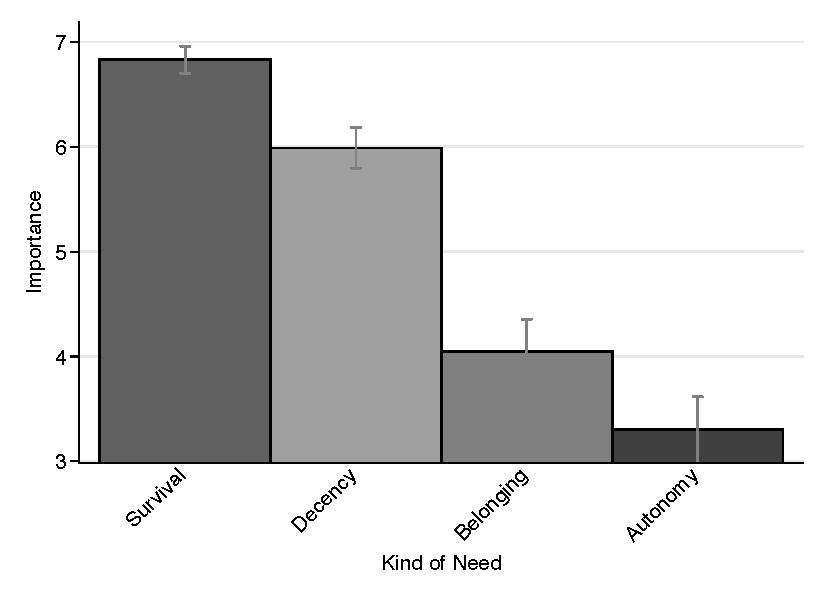
\includegraphics[width=0.5\linewidth]{figures/figure_15_english.pdf}}\\
   \textcolor{gray}{Evaluation}
\end{center}
\note{
   \begin{itemize}
      \item Wilcoxon signed-rank tests
      \item Ordered logistic regressions
   \end{itemize}
}
\end{frame}


%%%%%%%%%%%%
% SLIDE 35 %
%%%%%%%%%%%%
\begin{frame}{\vspace*{10mm}3.1\hspace*{1em}Study 1}
\textbf{Results (2/2)}\\
\medskip
\begin{itemize}
   \item Impartial observers assign different levels of importance to different kinds of needs
   \item Survival $>$ Decency $>$ Belonging $>$ Autonomy
\end{itemize}
\end{frame}


%%%%%%%%%%%%%%%%%%%%%%
% SLIDE 36 – STUDY 2 %
%%%%%%%%%%%%%%%%%%%%%%
\begin{frame}
\begin{overlayarea}{\textwidth}{0.81\paperheight}{
   \vspace*{11mm}
   \usebeamerfont{title}\textcolor{uolblue}
   {3.2\hspace*{1em}Study 2}
}
\end{overlayarea}
\end{frame}


%%%%%%%%%%%%
% SLIDE 37 %
%%%%%%%%%%%%
\begin{frame}{\vspace*{10mm}3.2\hspace*{1em}Study 2}
\textbf{Design and Implementation (1/2)}\\
\medskip
\begin{itemize}
   \item Respondi, online panel, April 2021
   \item $n=200$ (stratified as above)
   \item Impartial decision-makers
   \item $4$ kinds of needs (\textit{within subjects})
   \item $2\times7$ cases (\textit{within subjects})
   \begin{itemize}
      \item $6$ Mixed Cases
      \item $1$ Paired Case
   \end{itemize}
   \item $2$ Productivity Scenarios (\textit{within subjects})
   \begin{itemize}
      \item Equal Productivity Scenario ($\textsf{A}=\textsf{B}=500$, $\textsf{A}+\textsf{B}=1.000$)
      \item Unequal Productivity Scenario ($\textsf{A}=200$, $\textsf{B}=800$, $\textsf{A}+\textsf{B}=1.000$)
   \end{itemize}
\end{itemize}
\end{frame}


%%%%%%%%%%%%
% SLIDE 38 %
%%%%%%%%%%%%
\begin{frame}{\vspace*{10mm}3.2\hspace*{1em}Study 2}
\textbf{Design and Implementation (2/2)}\\
\medskip
\begin{center}
   \begin{tabular}{lcccccc}
      \arrayrulecolor{blue2}
      \hline
                 & \multicolumn{6}{c}{Case}                                                       \\
                 & 1          & 2           & 3          & 4           & 5          & 6           \\
      \hline\hline\\[-0.5em]
      A          & Survival   & Survival    & Survival   & Decency     & Decency    & Belonging   \\
      B          & Decency    & Belonging   & Autonomy   & Belonging   & Autonomy   & Autonomy    \\
      \hline
   \end{tabular}\\
   \smallskip
   \textcolor{gray}{Mixed Cases}
\end{center}
\end{frame}


%%%%%%%%%%%%
% SLIDE 39 %
%%%%%%%%%%%%
\begin{frame}{\vspace*{10mm}3.2\hspace*{1em}Study 2}
\textbf{Vignette (1/3)}\\
\medskip
\enquote{Please imagine two people with the names A and B.
A and B do not know each other.
Both are in need of wood.
The community of A and B allows them to chop wood in the community forest for a certain period of time.
Both have little money and therefore have no other way to get wood.\\
\medskip
On the coming pages, we will present you with a total of 14 cases where A and B need the wood for different reasons.
On each page, we will tell you what A needs the wood for and what B needs the wood for.
You will then be asked to divide the wood as fairly as possible between A and B.}
\end{frame}


%%%%%%%%%%%%
% SLIDE 40 %
%%%%%%%%%%%%
\begin{frame}{\vspace*{10mm}3.2\hspace*{1em}Study 2}
\textbf{Vignette (2/3)}\\
\medskip
\enquote{Please note that you have to make the following trade-off:
The more wood you give to one person, the less you can give to the other.
It is not possible to completely meet the needs of both people at the same time.
In each of the 14 cases, the available amount of wood will only be enough to completely cover the needs of one of the two people; the other person would then go away empty-handed.\\
\medskip
We now present to you the four different reasons for which A and B may need the wood.
These four reasons have to do with the coming winter.
Since you need to distribute the wood in advance without knowing exactly how cold the winter will be, we describe the expected effects of the winter on the people as more or less likely.\\
\medskip
Please read the descriptions of the four reasons carefully.}
\end{frame}


%%%%%%%%%%%%
% SLIDE 41 %
%%%%%%%%%%%%
\begin{frame}{\vspace*{10mm}3.2\hspace*{1em}Study 2}
\textbf{Vignette (3/3)}\\
\medskip
\begin{itemize}
   \item Same illustrations as in Study 1
   \item Slightly altered descriptions compared to Study 1
\end{itemize}
\medskip
\begin{multicols}{4}
   \begin{center}
      \frame{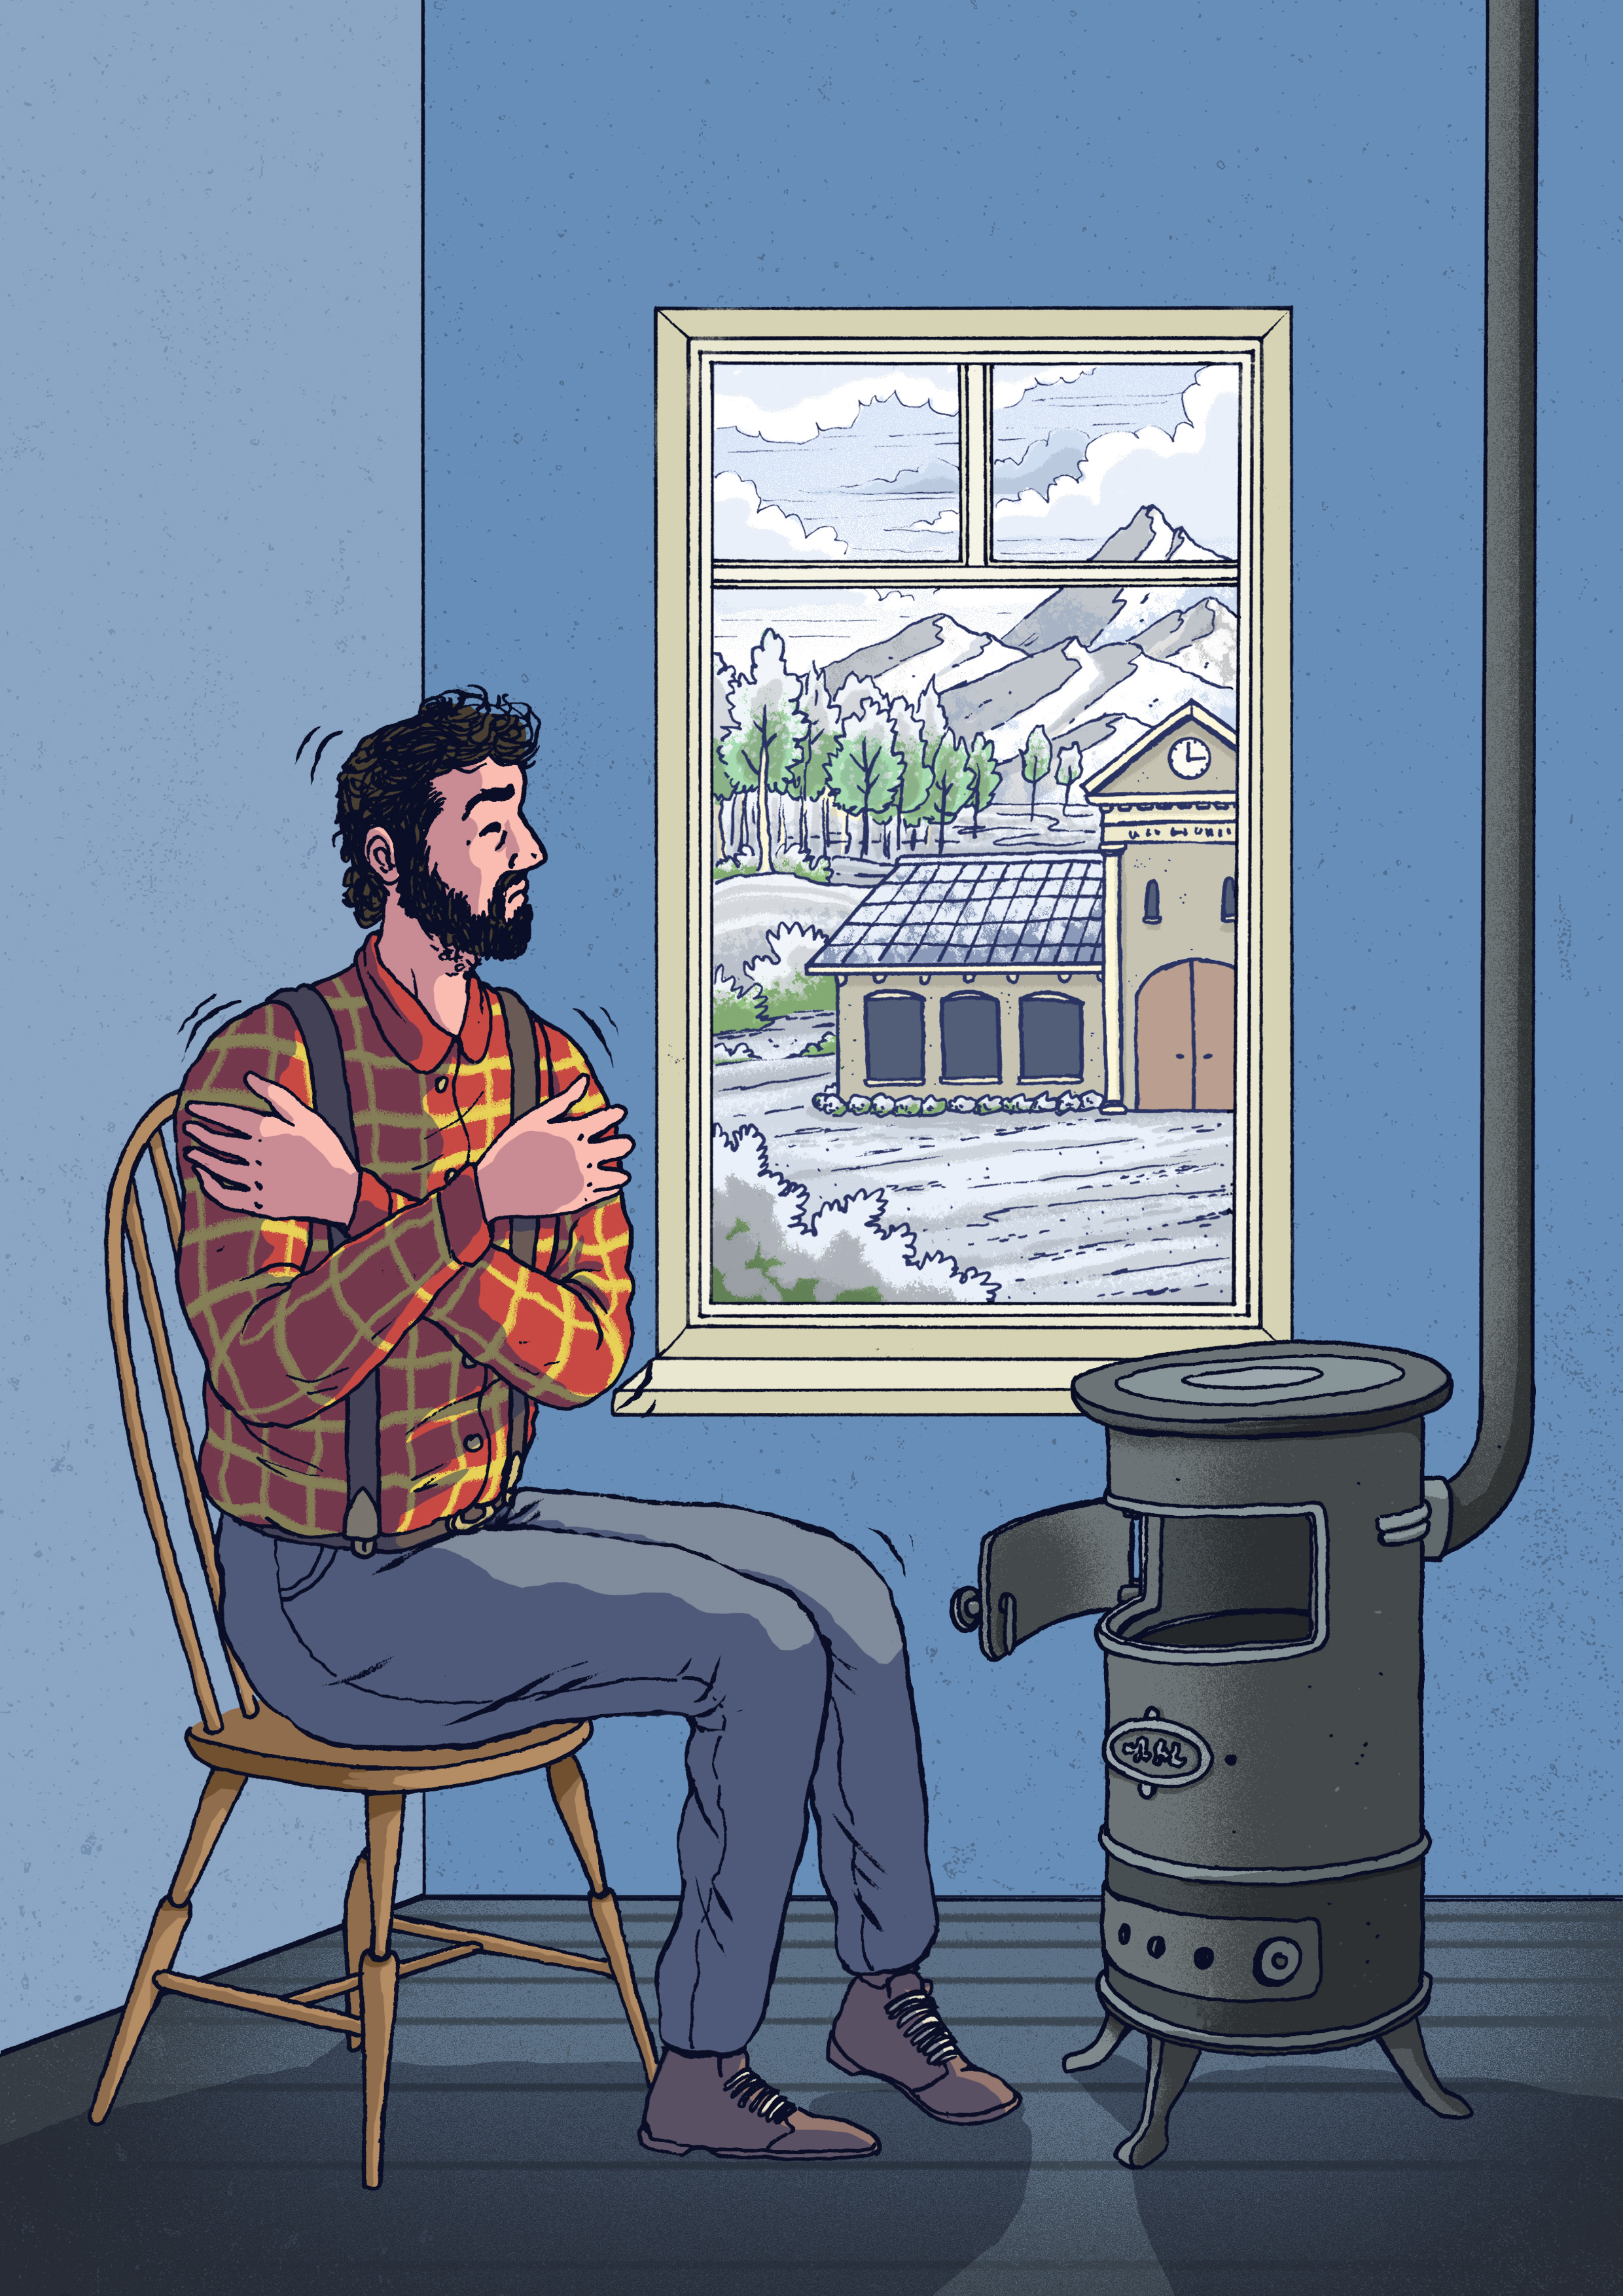
\includegraphics[width=0.8\linewidth]{figures/figure_11.jpg}}\\
      \textcolor{gray}{Illustration\\\textit{Survival}}\\
      \frame{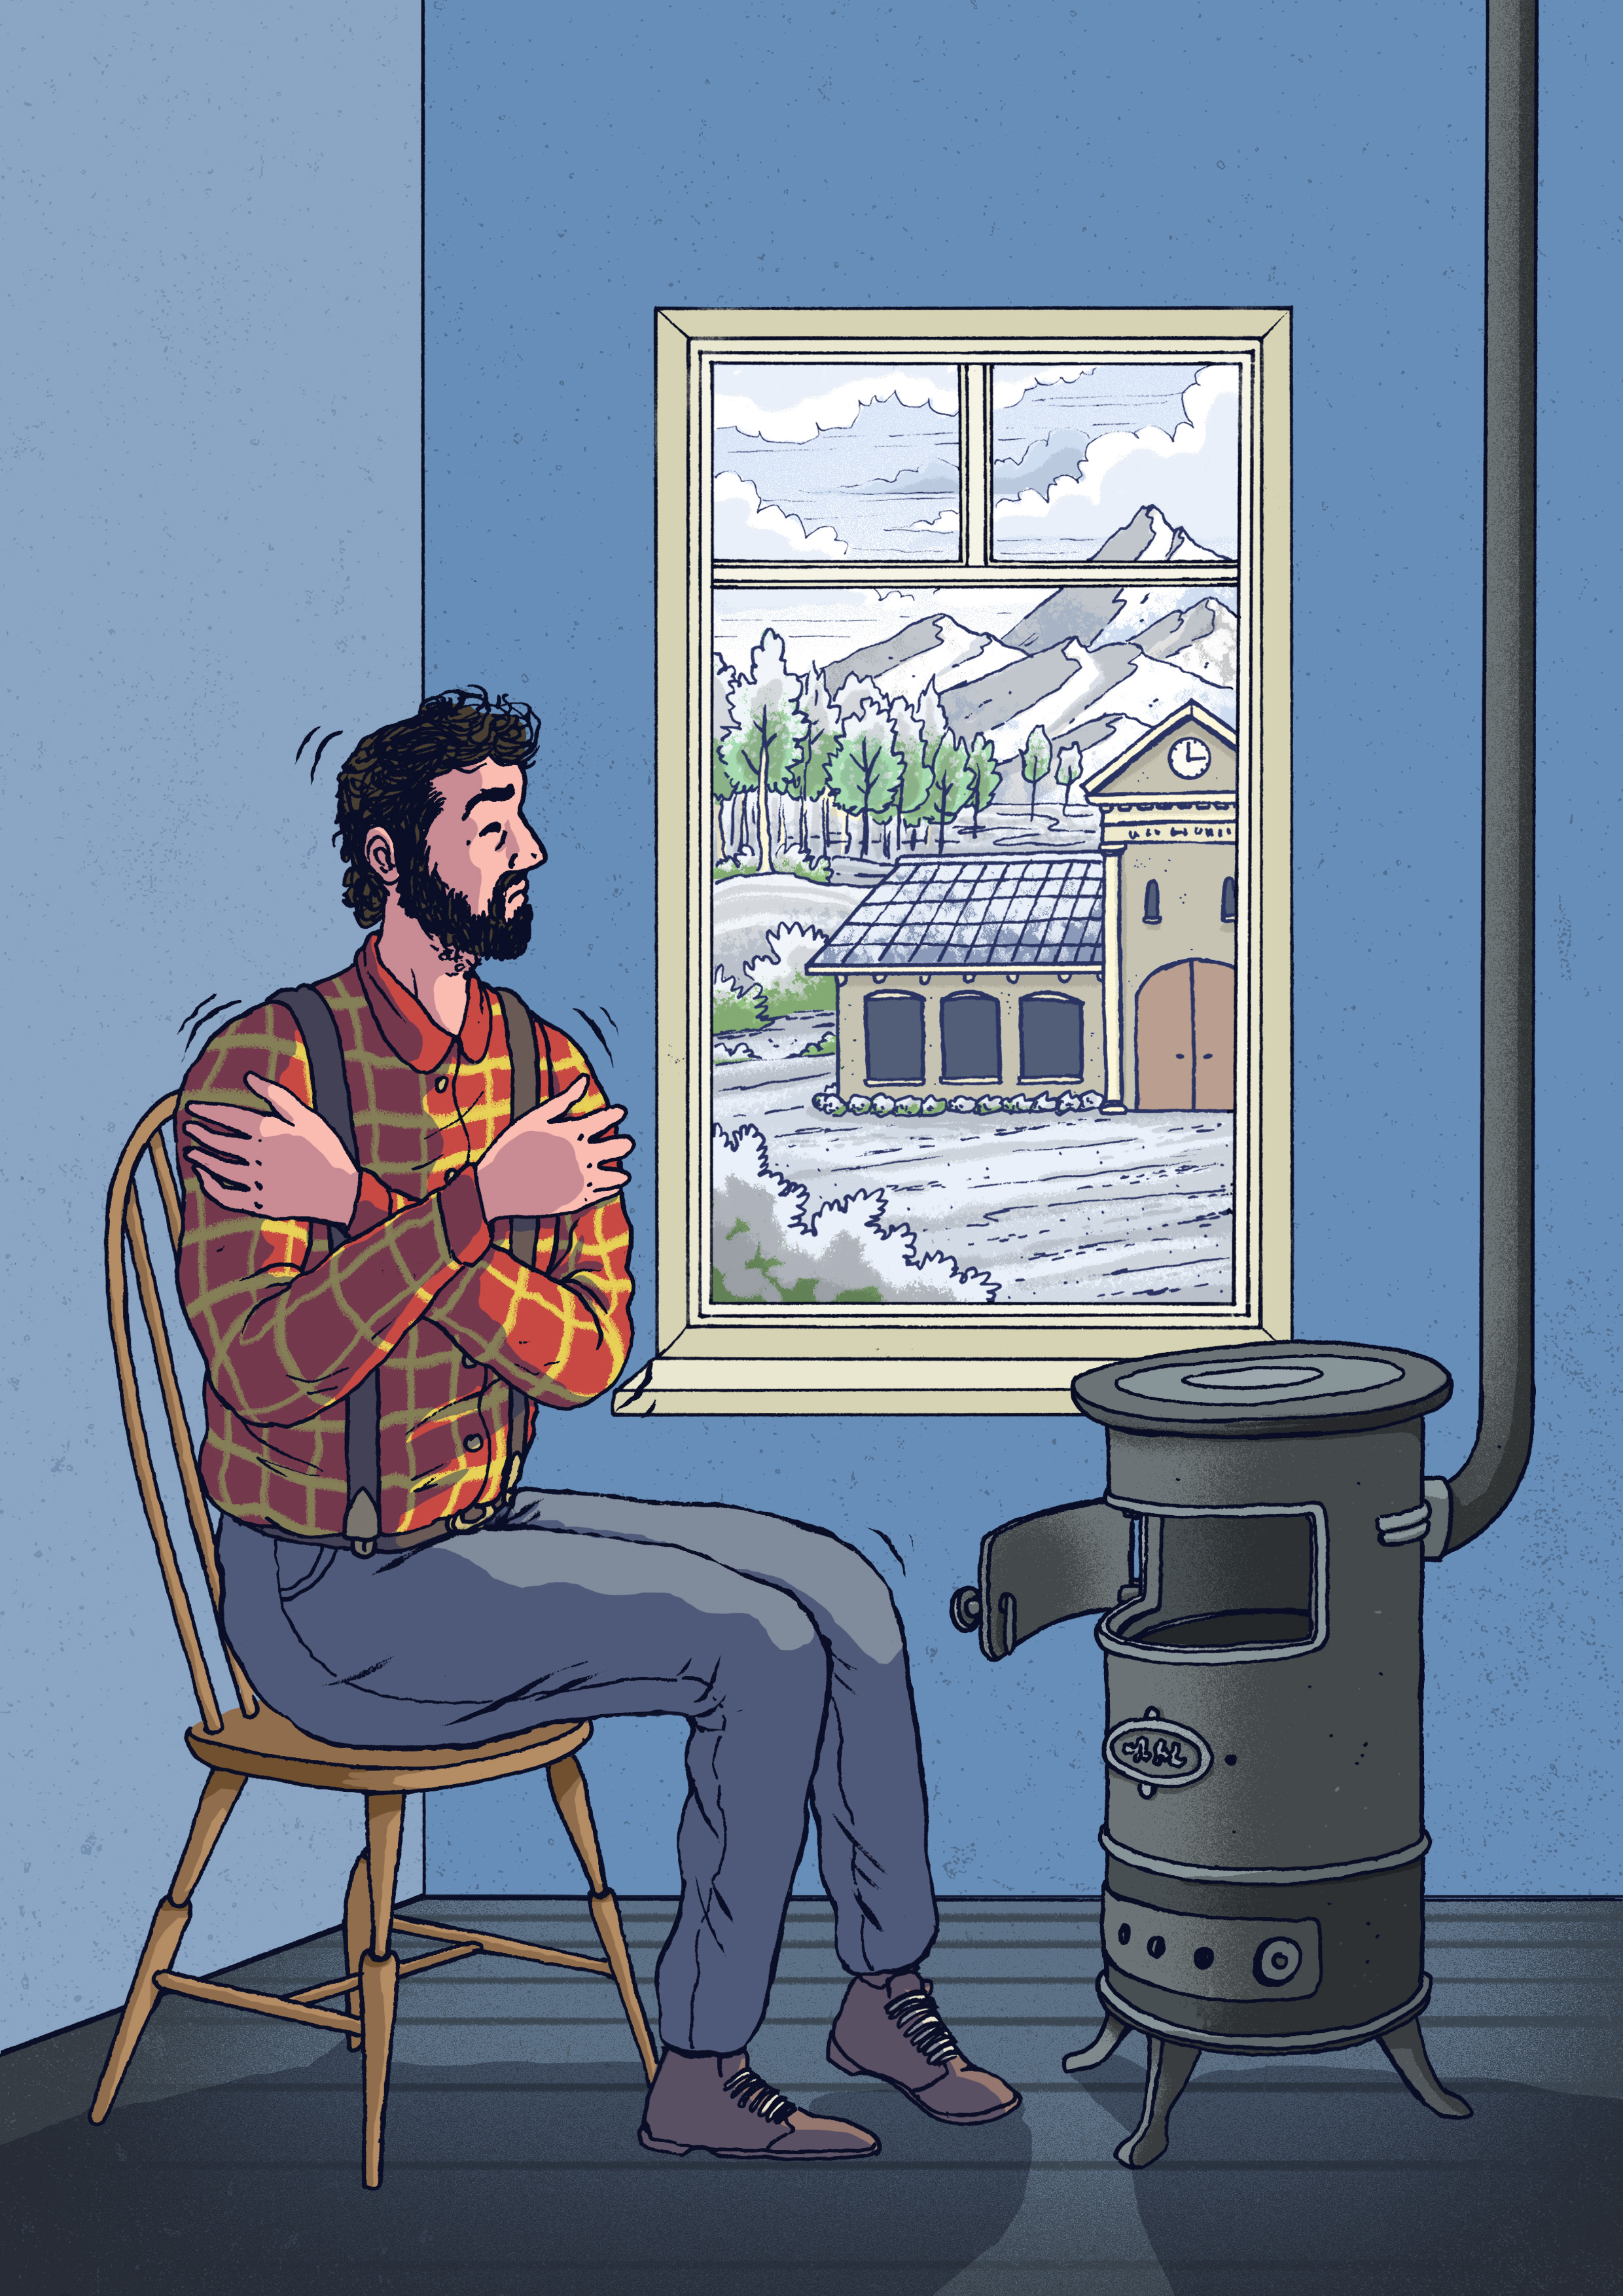
\includegraphics[width=0.8\linewidth]{figures/figure_12.jpg}}\\
      \textcolor{gray}{Illustration\\\textit{Decency}}\\
      \frame{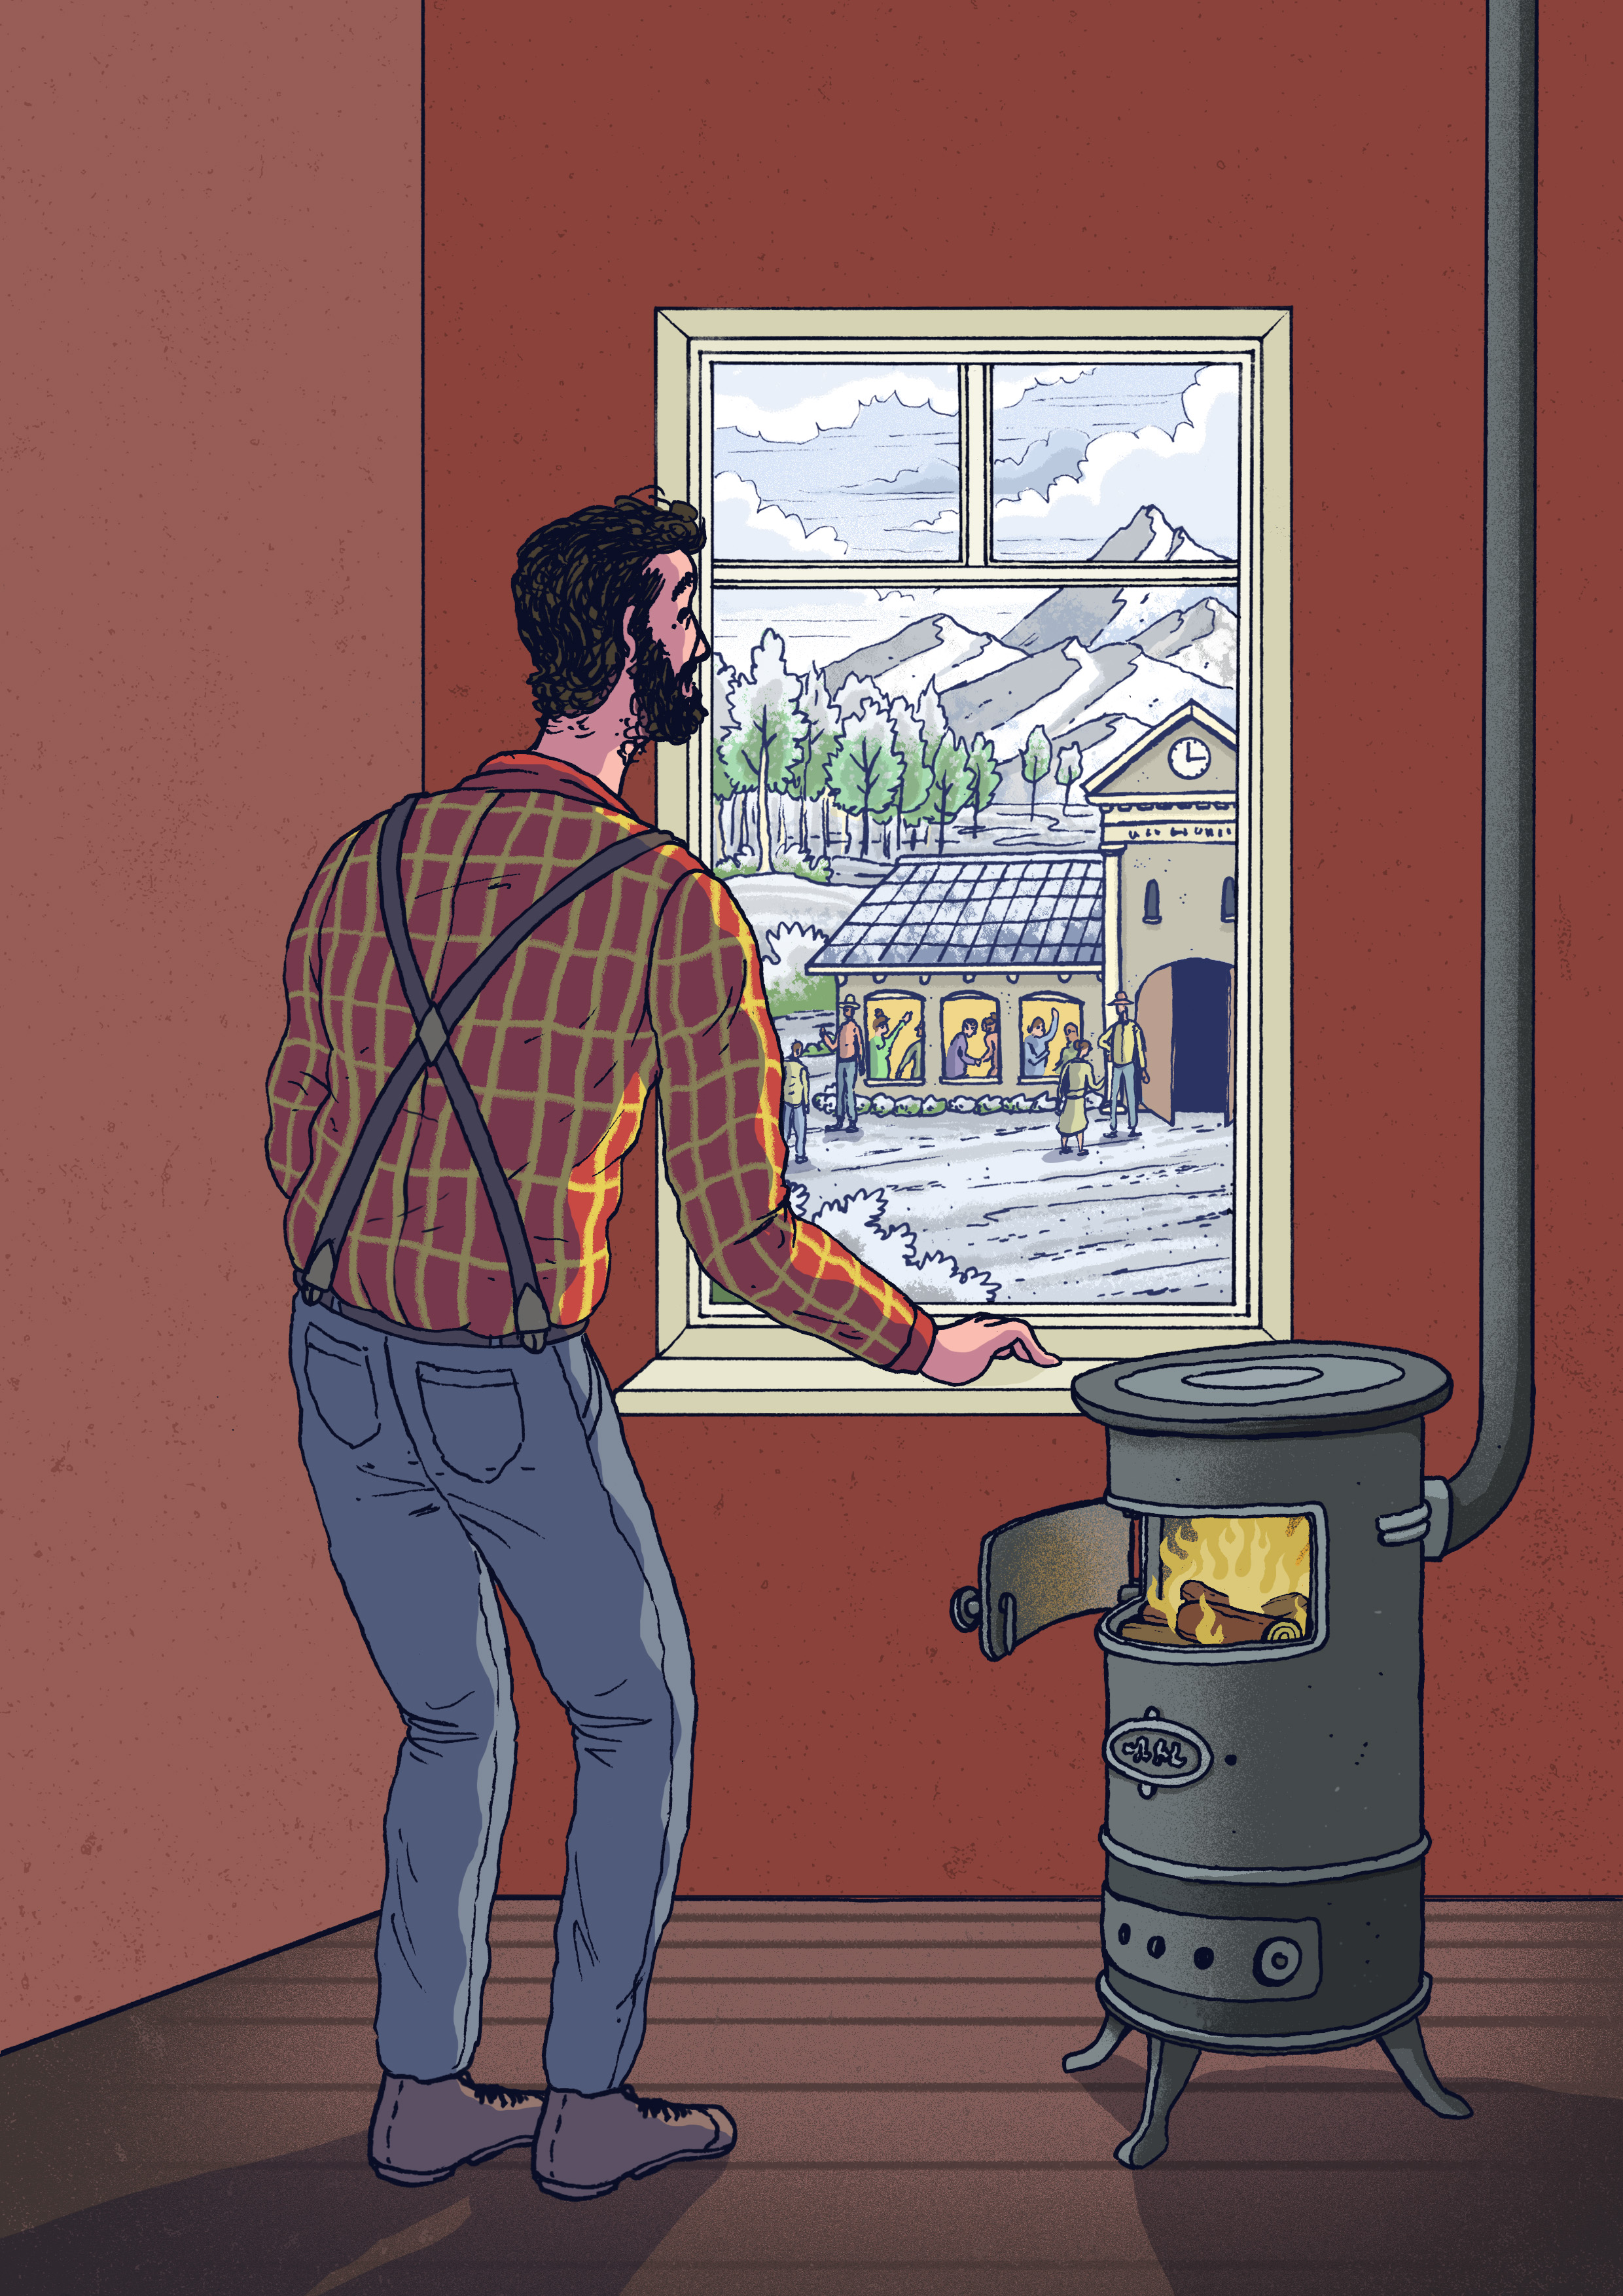
\includegraphics[width=0.8\linewidth]{figures/figure_13.jpg}}\\
      \textcolor{gray}{Illustration\\\textit{Belonging}}\\
      \frame{
\includegraphics[width=0.8\linewidth]{figures/figure_14.jpg}}\\
      \textcolor{gray}{Illustration\\\textit{Autonomy}}\\
   \end{center}
\end{multicols}
\end{frame}


%%%%%%%%%%%%
% SLIDE 42 %
%%%%%%%%%%%%
\begin{frame}{\vspace*{10mm}3.2\hspace*{1em}Study 2}
\textbf{Task}\\
\medskip
\begin{center}
   \frame{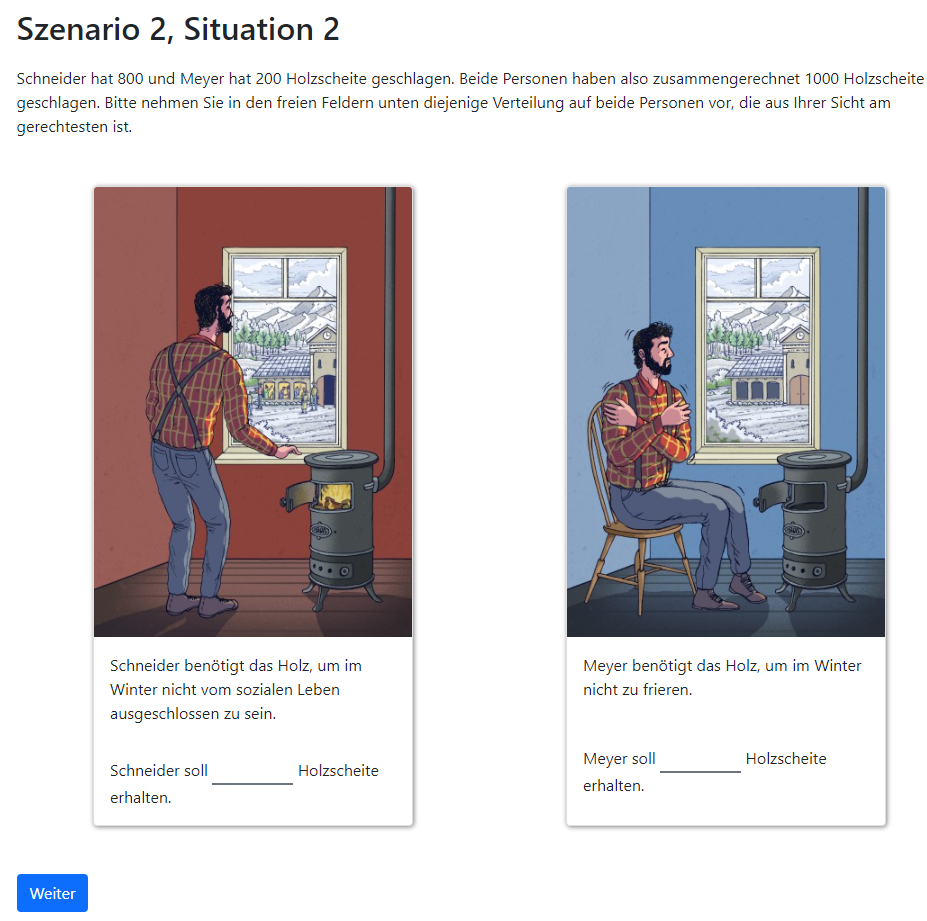
\includegraphics[width=0.4\linewidth]{figures/slides_otree_3.png}}\\
   \textcolor{gray}{Distribution Task \textit{Belonging -- Decency}}
\end{center}
\note{
   \begin{itemize}
      \item At the top, key information is summarized, e.\,g., who produced how much
      \item Below, the illustration is repeated together with a summary sentence
      \item At At the bottom, participants could enter how much each person should receive
   \end{itemize}
}
\end{frame}


%%%%%%%%%%%%
% SLIDE 43 %
%%%%%%%%%%%%
\begin{frame}{\vspace*{10mm}3.2\hspace*{1em}Study 2}
\textbf{Results (1/4)}\\
\medskip
\begin{center}
   $\Delta_{\alpha,\beta}=\gamma_{A}-\gamma_{B}$
\end{center}
\note{
   \begin{itemize}
      \item Examples: $A=600,B=400,\Delta=200$, $A=400,B=600,\Delta=-200$
   \end{itemize}
}
\end{frame}


%%%%%%%%%%%%
% SLIDE 44 %
%%%%%%%%%%%%
\begin{frame}{\vspace*{10mm}3.2\hspace*{1em}Study 2}
\textbf{Results (2/4)}\\
\medskip
\begin{center}
   \frame{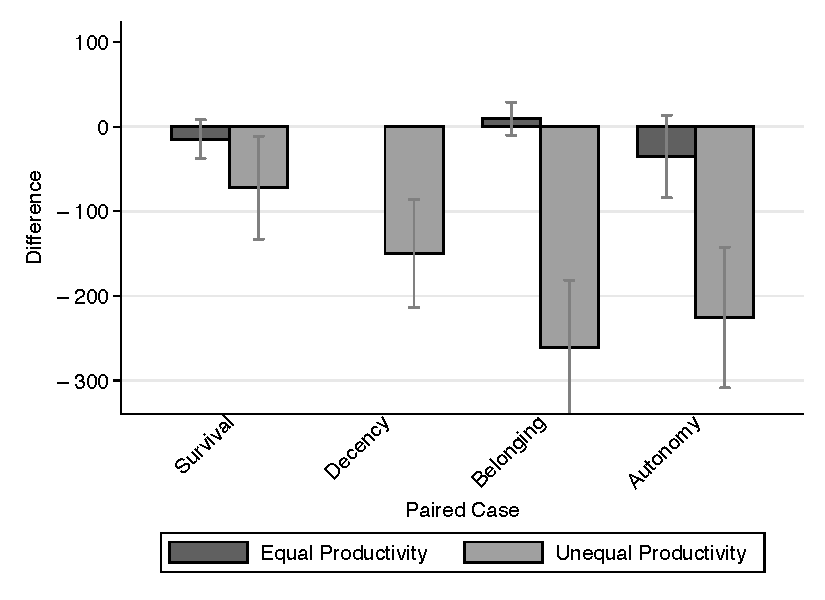
\includegraphics[width=0.5\linewidth]{figures/figure_16_english.pdf}}\\
   \textcolor{gray}{Differences of Paired Cases}
\end{center}
\note{
   \begin{itemize}
      \item Approximate equal distribution with equal productivity (two-sided Welch tests)
      \item Lower allocation to Person $A$ in cases of unequal productivity, but still more wood than they chopped themselves ($\Delta=200-800=-600$); in the case of \textit{Survival}, close to equal distribution (two-sided Welch tests)
   \end{itemize}
}
\end{frame}


%%%%%%%%%%%%
% SLIDE 45 %
%%%%%%%%%%%%
\begin{frame}{\vspace*{10mm}3.2\hspace*{1em}Study 2}
\textbf{Results (3/4)}\\
\medskip
\begin{center}
   \frame{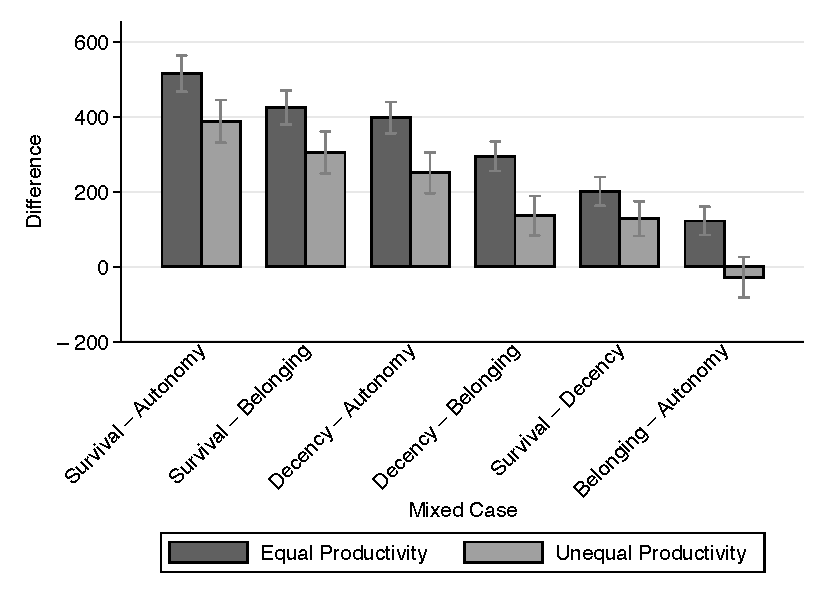
\includegraphics[width=0.5\linewidth]{figures/figure_17_english.pdf}}\\
   \textcolor{gray}{Differences of Mixed Cases}
\end{center}
\note{
   \begin{itemize}
      \item Difference is smaller in cases of unequal productivity (two-sided Welch tests)
      \item More wood than chopped themselves (except in the last bar)
      \item Confirms the hierarchy from Study 1 (two-sided Welch tests)
      \begin{itemize}
         \item Four kinds of needs: greatest difference (\textit{Survival -- Autonomy})
         \item Three kinds of needs: moderate differences (\textit{Survival -- Belonging}, \textit{Decency -- Autonomy})
         \item Adjacent kinds of needs: smallest differences (\textit{Survival -- Decency}, \textit{Decency -- Belonging}, \textit{Belonging -- Autonomy})
      \end{itemize}
      \item Formulations make no difference (Tobit panel regressions)
   \end{itemize}
}
\end{frame}


%%%%%%%%%%%%
% SLIDE 46 %
%%%%%%%%%%%%
\begin{frame}{\vspace*{10mm}3.2\hspace*{1em}Study 2}
\textbf{Results (4/4)}\\
\medskip
\begin{itemize}
   \item \textcolor{gray}{Impartial} decision-makers \textcolor{gray}{assign different levels of importance to different kinds of needs}
   \item \textcolor{gray}{Survival $>$ Decency $>$ Belonging $>$ Autonomy}
   \item Decisions are influenced by productivity
\end{itemize}
\end{frame}


%%%%%%%%%%%%%%%%%%%%%%%%%%%%%%%%%%%%%
% SLIDE 47 – SUMMARY OF KEY RESULTS %
%%%%%%%%%%%%%%%%%%%%%%%%%%%%%%%%%%%%%
\begin{frame}
\begin{overlayarea}{\textwidth}{0.81\paperheight}{
   \vspace*{11mm}
   \usebeamerfont{title}\textcolor{uolblue}
   {4\hspace*{1em}Summary of Key Results}
}
\end{overlayarea}
\end{frame}


%%%%%%%%%%%%
% SLIDE 48 %
%%%%%%%%%%%%
\begin{frame}{\vspace*{10mm}4\hspace*{1em}Summary of Key Results}
\textbf{Need as Reference Point}
\medskip
\begin{itemize}
   \item[(1)] Impartial observers make gradual justice evaluations
   \item[(2)] Evaluations depend on supply situations
   \item[(3)] Evaluations are influenced by information on need
\end{itemize}
\end{frame}


%%%%%%%%%%%%
% SLIDE 49 %
%%%%%%%%%%%%
\begin{frame}{\vspace*{10mm}4\hspace*{1em}Summary of Key Results}
\textbf{Need and Accountability}\\
\medskip
\begin{itemize}
   \item[(4)] Impartial decision-makers take need, productivity, and accountability into account
   \item[(5)] Even in cases of low productivity, need is partially compensated
   \item[(6)] Willingness to compensate decreases when low productivity or high need is self-inflicted
\end{itemize}
\end{frame}


%%%%%%%%%%%%
% SLIDE 50 %
%%%%%%%%%%%%
\begin{frame}{\vspace*{10mm}4\hspace*{1em}Summary of Key Results}
\textbf{Kinds of Needs}\\
\medskip
\begin{itemize}
   \item[(7)] Impartial observers and decision-makers assign different levels of importance to different kinds of needs
   \item[(8)] Survival $>$ Decency $>$ Belonging $>$ Autonomy
\end{itemize}
\end{frame}


%%%%%%%%%%%%%%%%%%%%%%%%%%%%%%%%%%%%%%%%%
% SLIDE 51 – IF YOU WANT TO DIVE DEEPER %
%%%%%%%%%%%%%%%%%%%%%%%%%%%%%%%%%%%%%%%%%
\begin{frame}{\vspace*{10mm}If You Want to Dive Deeper$\ldots$}
\begin{multicols}{2}
   \begin{center}
      \frame{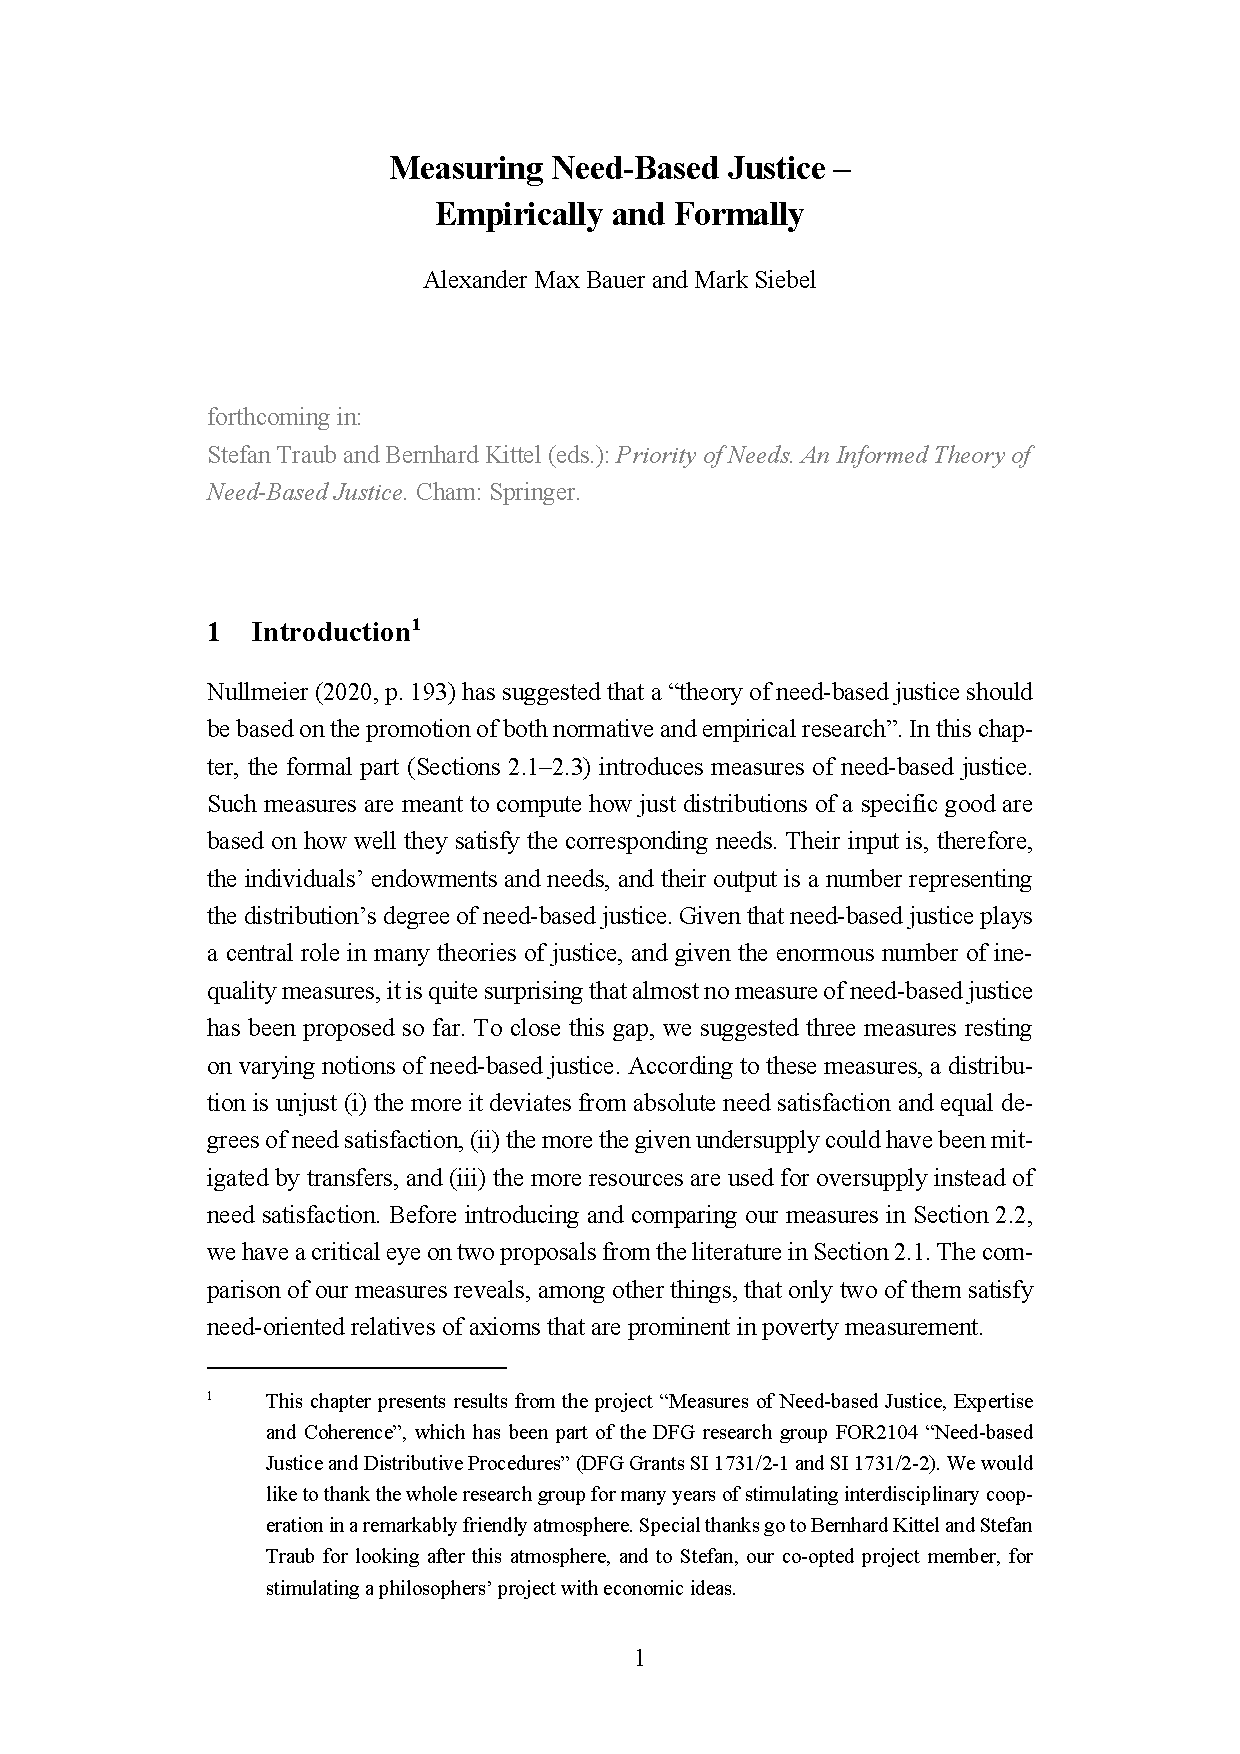
\includegraphics[width=0.5\linewidth]{figures/slides_bauer_siebel_nd.pdf}}\\
      \textcolor{gray}{Bauer and Siebel 2024}
      \frame{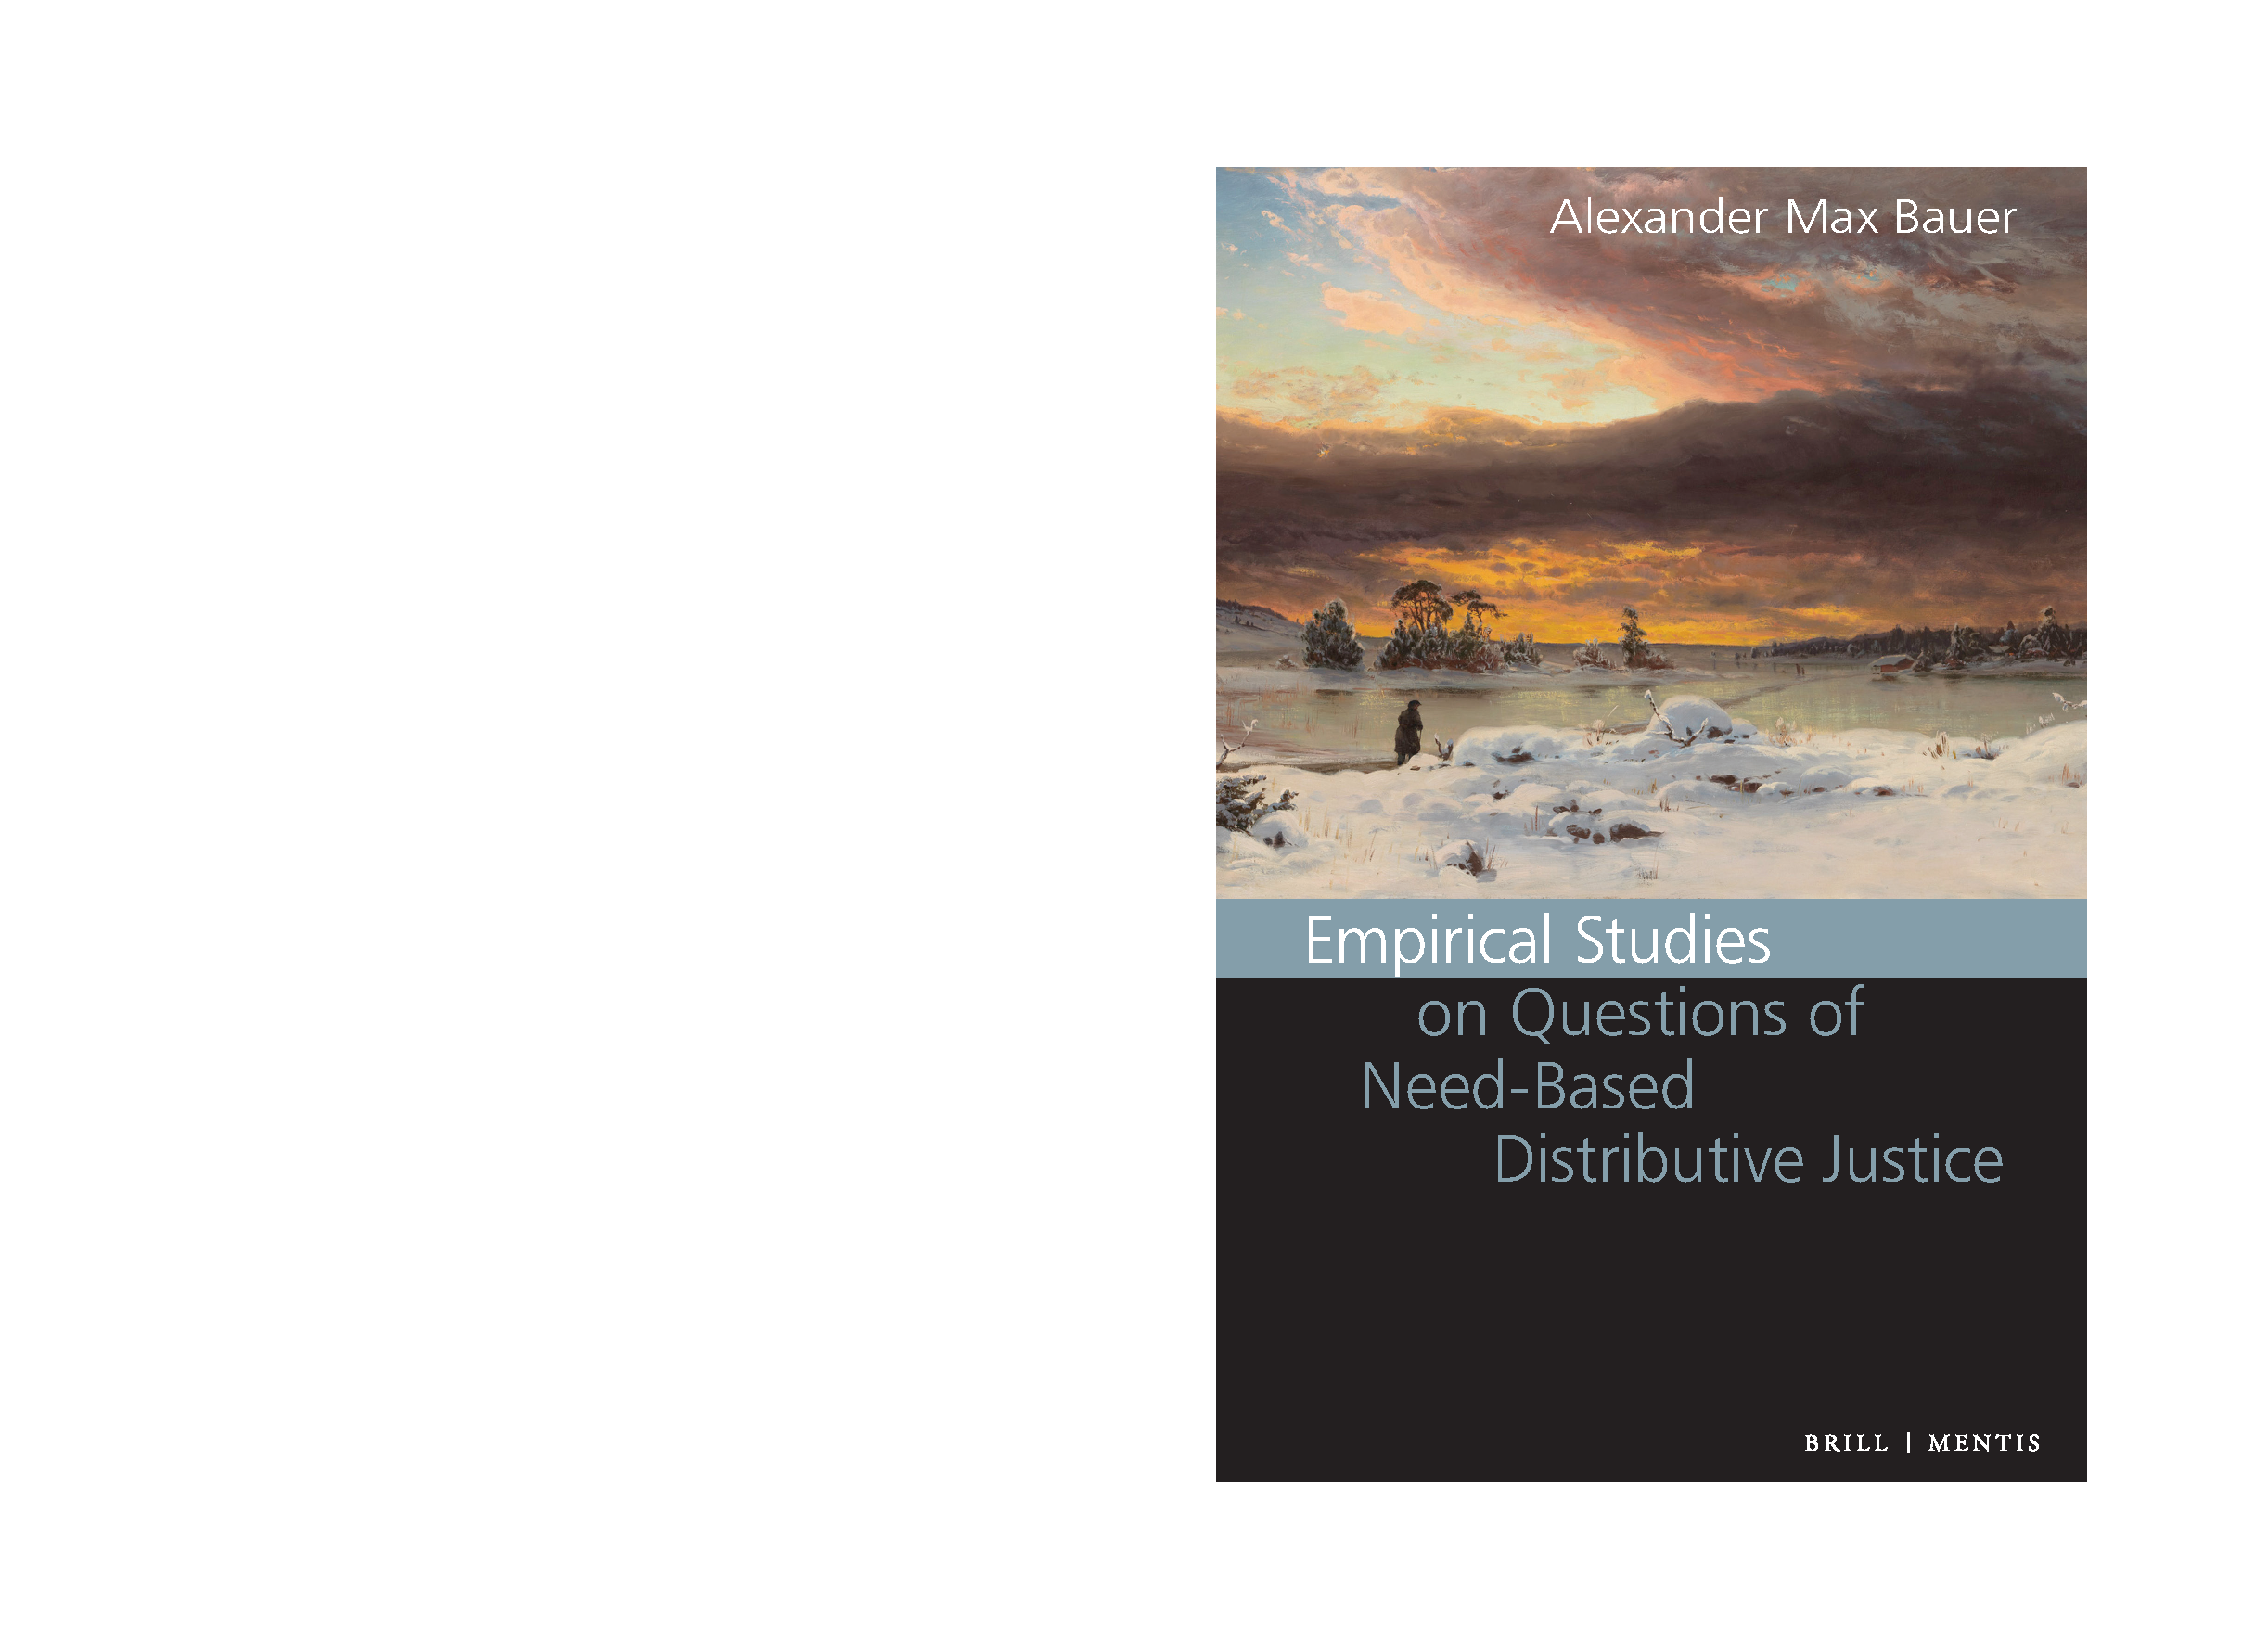
\includegraphics[width=0.5\linewidth]{figures/slides_bauer_forthcoming.pdf}}\\
      \textcolor{gray}{Bauer forthcoming}
   \end{center}
\end{multicols}
\begin{center}
   \textcolor{blue1}{Get in touch!}\\
   \textcolor{blue1}{http://alexandermaxbauer.net/}
   \bigskip
\end{center}
\note{
   \begin{itemize}
      \item Bauer, Alexander Max, and Mark Siebel (2024): \enquote{Measuring Need-Based Distributive Justice -- Formally and Empirically,} in: Bernhard Kittel and Stefan Traub (eds.): \textit{Priority of Needs? An Informed Theory of Need-Based Justice}, Cham: Springer, 59--91.
         \item Bauer, Alexander Max (forthcoming): \textit{Empirical Studies on Questions of Need-Based Distributive Justice}, Paderborn: Brill $|$ mentis.
   \end{itemize}
}
\end{frame}


%%%%%%%%%%%%%%%%%%%%%
% SLIDE 52 – THANKS %
%%%%%%%%%%%%%%%%%%%%%
\begin{frame}{}
\begin{center}
   
\includegraphics[width=0.8\linewidth]{figures/slides_thanks_english.pdf}
\end{center}
\end{frame}


%%%%%%%%%%%%%%%%%%%%%%%%%
% SLIDE 53 – LITERATURE %
%%%%%%%%%%%%%%%%%%%%%%%%%
\begin{frame}{\vspace*{10mm}Literature}
\vspace*{-5mm}
{\footnotesize
\begin{itemize}[label=,leftmargin=2em,itemindent=-2em]
   \item Bauer, Alexander Max, Frauke Meyer, Jan Romann, Mark Siebel, and Stefan Traub (2022): \enquote{Need, Equity, and Accountability. Evidence on Third-Party Distributive Decisions from a Vignette Study,} \textit{Social Choice and Welfare} 59, 769--814.
   \item Bauer, Alexander Max, Jan Romann, Mark Siebel, and Stefan Traub (2023): \enquote{Winter is Coming. How Laypeople Think About Different Kinds of Needs,} \textit{PLOS ONE} 18 (11), e0294572.
   \item Bauer, Alexander Max, and Jan Romann (2024): \enquote{Equal Deeds, Different Needs. Need, Accountability, and Resource Availability in Third-Party Distributive Decisions,} in: Shaun Nichols and Joshua Knobe (eds.): \textit{Oxford Studies in Experimental Philosophy}, vol. 5, Oxford: Oxford University Press, 7--31.
   \item Bauer, Alexander Max, and Mark Siebel (2024): \enquote{Measuring Need-Based Distributive Justice -- Formally and Empirically,} in: Bernhard Kittel and Stefan Traub (eds.): \textit{Priority of Needs? An Informed Theory of Need-Based Justice}, Cham: Springer, 59--91.
   \item Bauer, Alexander Max (forthcoming): \textit{Empirical Studies on Questions of Need-Based Distributive Justice}, Paderborn: Brill $|$ mentis.
   \item Bauer, Alexander Max, Adele Diederich, Stefan Traub, and Arne Robert Weiss (forthcoming): \enquote{Thinking About Need. A Vignette Experiment on Need-Based Distributive Justice,} \textit{The Journal of Economic Inequality}.
\end{itemize}
}
\end{frame}


\end{document}
